%!TEX TS-program = xelatex

% HSE Beamer Theme
% by Danil Fedorovykh
% http://hse.ru/staff/df
%
% Version 2.0 (English)
% January 2022

%%% Set up the free HSE Sans font
%%% https://www.hse.ru/info/brandbook/#font

\documentclass[aspectratio=169]{beamer}

\newbool{russian}
\booltrue{russian} % Uncomment if in Russian
\usepackage{HSE-theme/beamerthemeHSE} % Load HSE theme
\usepackage[no-math]{fontspec}      % fonts loading
\usepackage{caption}
\usepackage{subfigure}
\usepackage{subcaption}
\usepackage{hyperref}
\usepackage[dvipsnames]{xcolor}
\usepackage{ragged2e}
\captionsetup[figure]{labelformat=empty}
\captionsetup[subfigure]{labelformat=empty}
\setsansfont{HSE Sans}
%\graphicspath{{./images/}}
\graphicspath{{/home/llyy/Yandex.Disk/personal/knowledge/general/algorithms_course/repo/algorithms_course/0_intro/slides/images}}


%%% Информация об авторе и выступлении
\title[Title]{Алгоритмы и структуры данных} 
\subtitle{Лекция 0. Алгоритмы, вычислительные машины и программы}
\author[Author's name]{Илья Сергеевич Бычков\\ \smallskip \scriptsize \url{ibychkov@hse.ru}}
\institute{НИУ ВШЭ - Нижний Новгород}
\date{\today}


\begin{document}

\frame[plain]{\titlepage}


%%%%%%%%%%%%%%%%%%%%%%%%%%%%%%%%%%%%%%%%%%%%%%%%%%%%%%%%%%%%%%%%%%%%%%%%%%%%%%%%%%%%%%%%%%%%%%%%%%
\begin{frame}[c]
%\frametitle{A first slide}

\begin{center}
\Huge О курсе
\end{center}

\end{frame}
%%%%%%%%%%%%%%%%%%%%%%%%%%%%%%%%%%%%%%%%%%%%%%%%%%%%%%%%%%%%%%%%%%%%%%%%%%%%%%%%%%%%%%%%%%%%%%%%%%

\begin{frame}
\frametitle{О курсе}
\framesubtitle{Организационная информация}

Продолжительность курса: \quad октябрь - июнь / 2-4 модули /9 месяцев\newline
Состав курса: \quad примерно 30 лекций + 30 практик\newline

Результаты курса: 2 оценки  - оценка за модуль 2 и итоговая оценка\newline

Оценка модуль 2 = Накопленная оценка (2) * 0.6 + Экзамен (2)* 0.4\newline
Оценка модули 3-4 = Накопленная оценка (3-4) * 0.6 + Экзамен (3-4) * 0.4\newline
Финальная оценка = Оценка (2) * 0.4 + Оценка (3-4) * 0.6\newline

Из чего складывается накопленная оценка:
\begin{itemize}
  \item{Контесты - \textcolor{red}{вес 0.3}}
  \item{Контрольные - \textcolor{red}{вес 0.6, блокирующий элемент}}
  \item{Активность/доп задания - \textcolor{red}{вес 0.1}}
\end{itemize}
\end{frame}

%%%%%%%%%%%%%%%%%%%%%%%%%%%%%%%%%%%%%%%%%%%%%%%%%%%%%%%%%%%%%%%%%%%%%%%%%%%%%%%%%%%%%%%%%%%%%%%%%%

\begin{frame}
\frametitle{О курсе}
\framesubtitle{Команда курса}
Лекции:
\begin{itemize}
\item{\textcolor{blue}{Илья Сергеевич Бычков} - HSE PhD, Senior Algorithm Developer (Huawei), старший научный сотрудник ЛАТАС}
\end{itemize}
Семинары:
\begin{itemize}
  \item{\textcolor{blue}{Максим Отчество Захаров} - Intel, Yadro}
  \item{\textcolor{blue}{Михаил Михайлович Железин} - Yandex}
  \item{\textcolor{blue}{Никита Александрович Наумов} - Sber}
  \item{\textcolor{blue}{Кирилл Сергеевич Тараканов} - Huawei, ШАД}
\end{itemize}
\end{frame}

\begin{frame}
\frametitle{О курсе}
\framesubtitle{План курса}
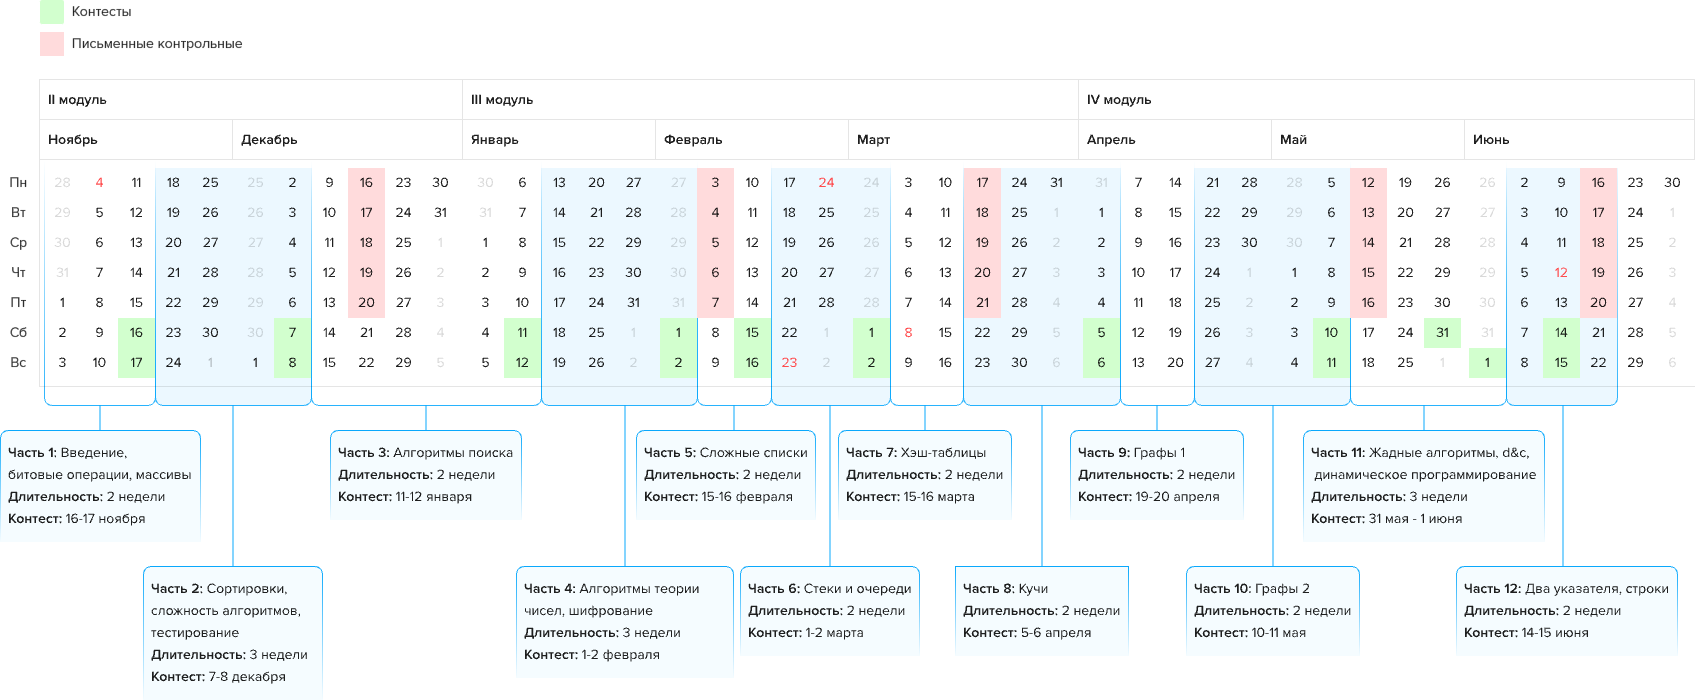
\includegraphics[width=1.05\textwidth]{schedule}
\end{frame}

%%%%%%%%%%%%%%%%%%%%%%%%%%%%%%%%%%%%%%%%%%%%%%%%%%%%%%%%%%%%%%%%%%%%%%%%%%%%%%%%%%%%%%%%%%%%%%%%%%

\begin{frame}
\frametitle{О курсе}
\framesubtitle{Литература}
\begin{figure}
    \captionsetup[subfigure]{labelformat=empty}
    \centering
    \subfigure[\textbf{\newline Introduction to \newline Algorithms, 4th Edition}\newline Thomas H Cormen \newline Charles E Leiserson \newline Ronald L Rivest \newline Clifford Stein]{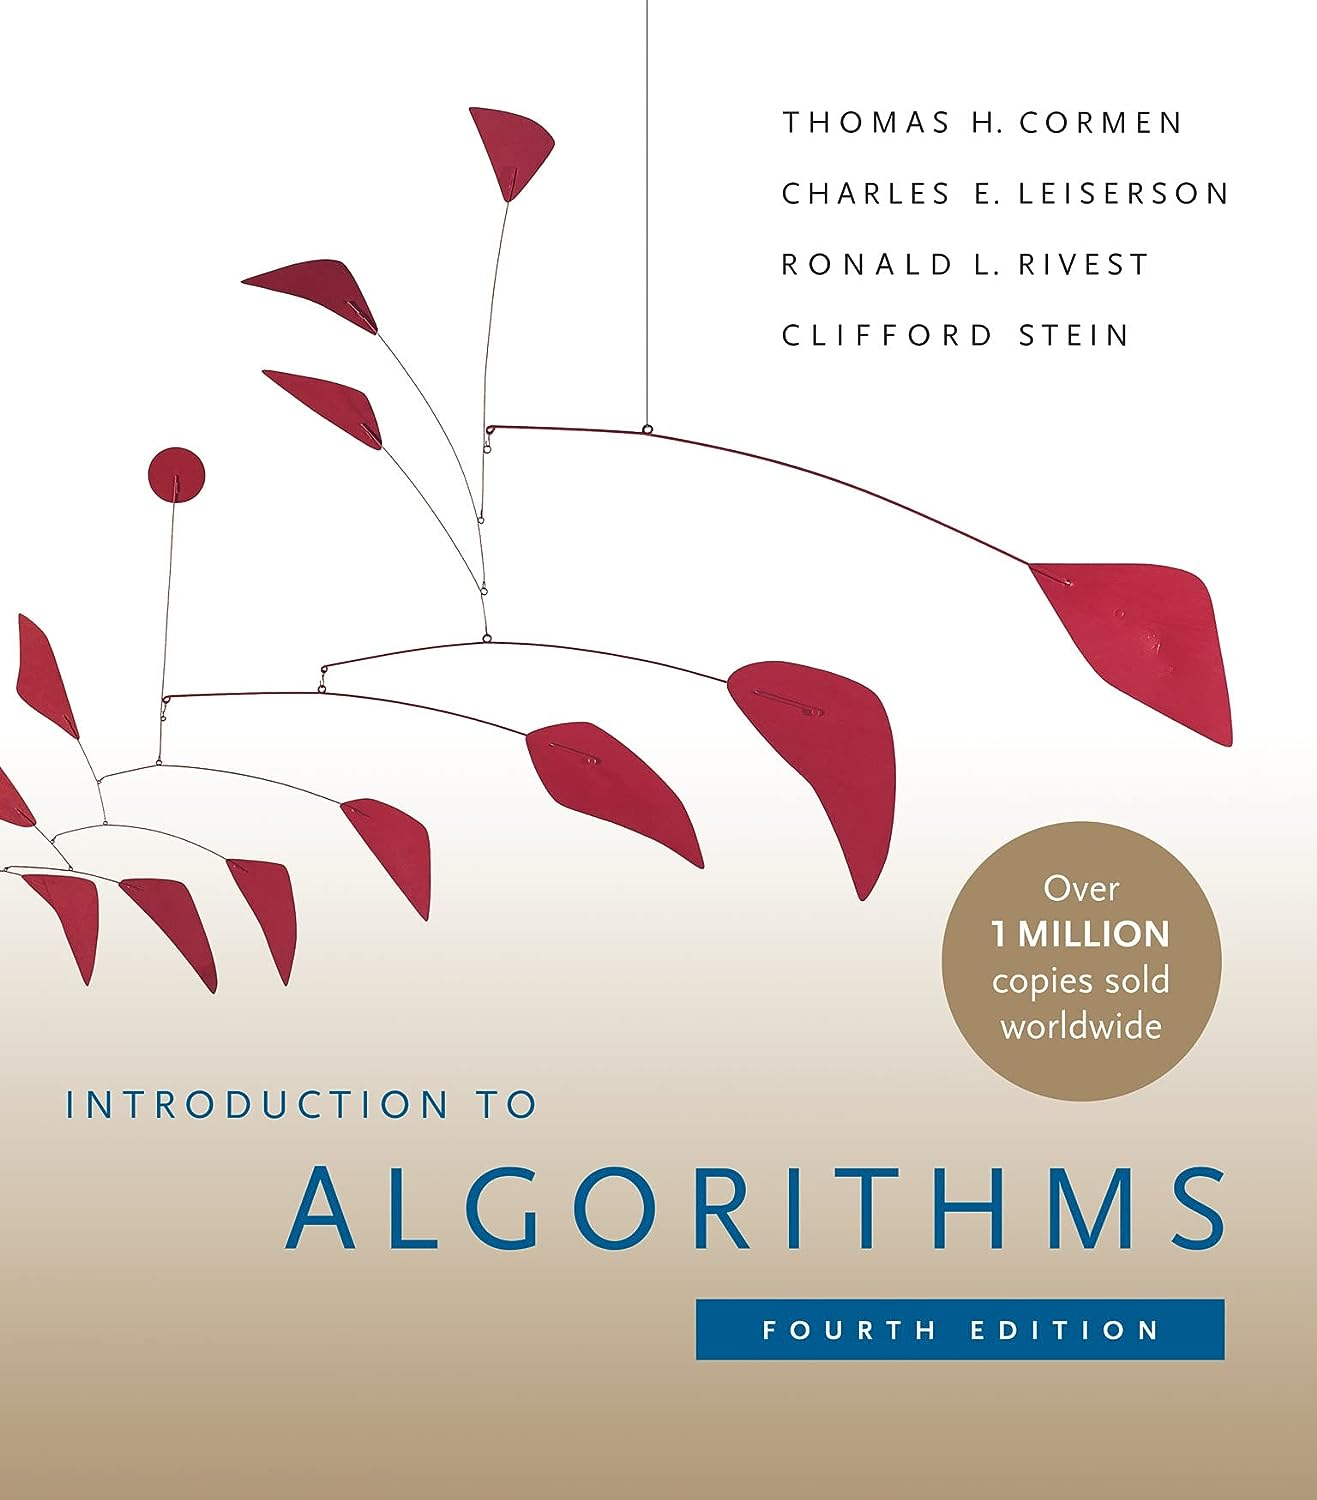
\includegraphics[width=0.24\textwidth]{cormen_4_cover}} 
    \subfigure[\textbf{\newline Algorithms}\newline Sanjoy Dasgupta \newline Christos Papadimitriou \newline Umesh Vazirani ]{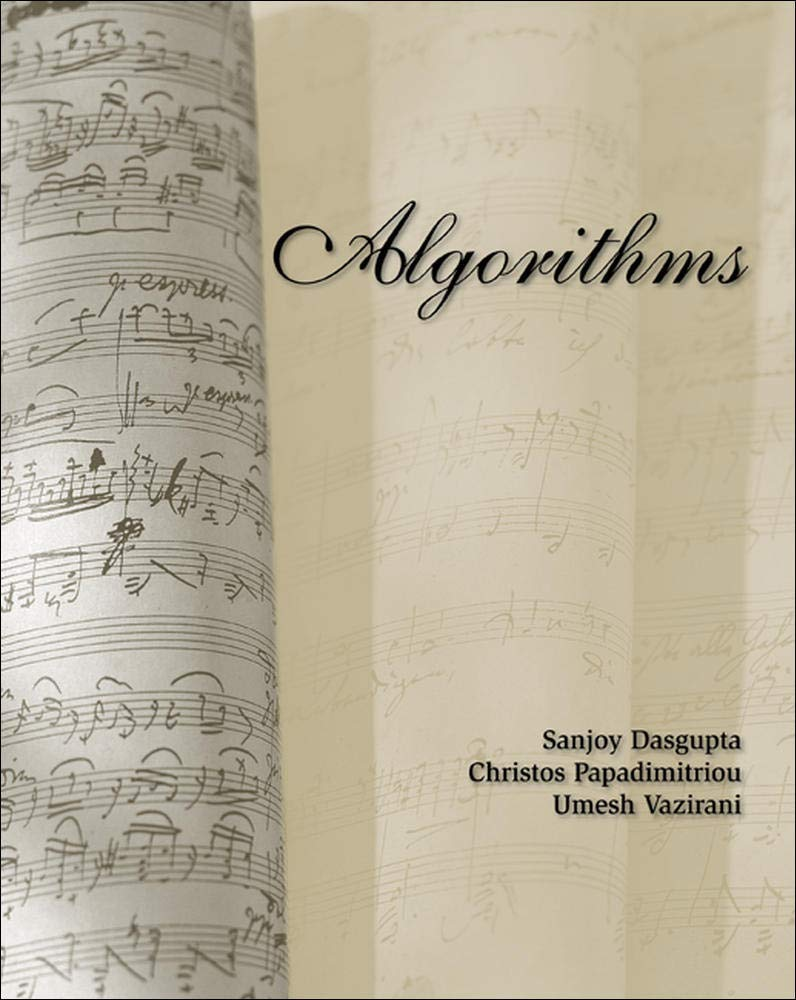
\includegraphics[width=0.24\textwidth]{dasgupta_cover}} 
    \subfigure[\textbf{\newline Algorithms, 4th Edition}\newline Robert Sedgewick \newline Kevin Wayne\newline \newline \url{algs4.cs.princeton.edu}]{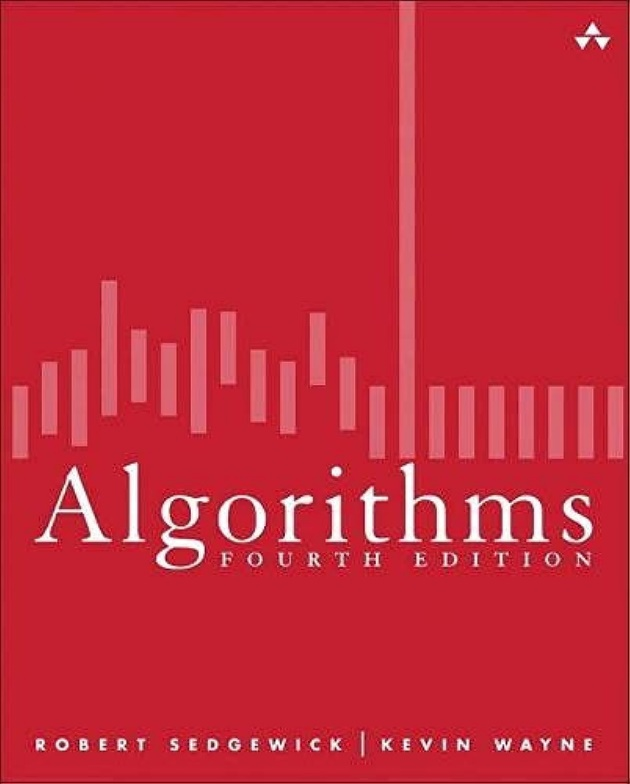
\includegraphics[width=0.24\textwidth]{sedgewick_cover}} 
    \subfigure[\textbf{Introduction to Algorithms, 4th Edition}\newline Thomas H Cormen, Charles E Leiserson, Ronald L Rivest, Clifford Stein]{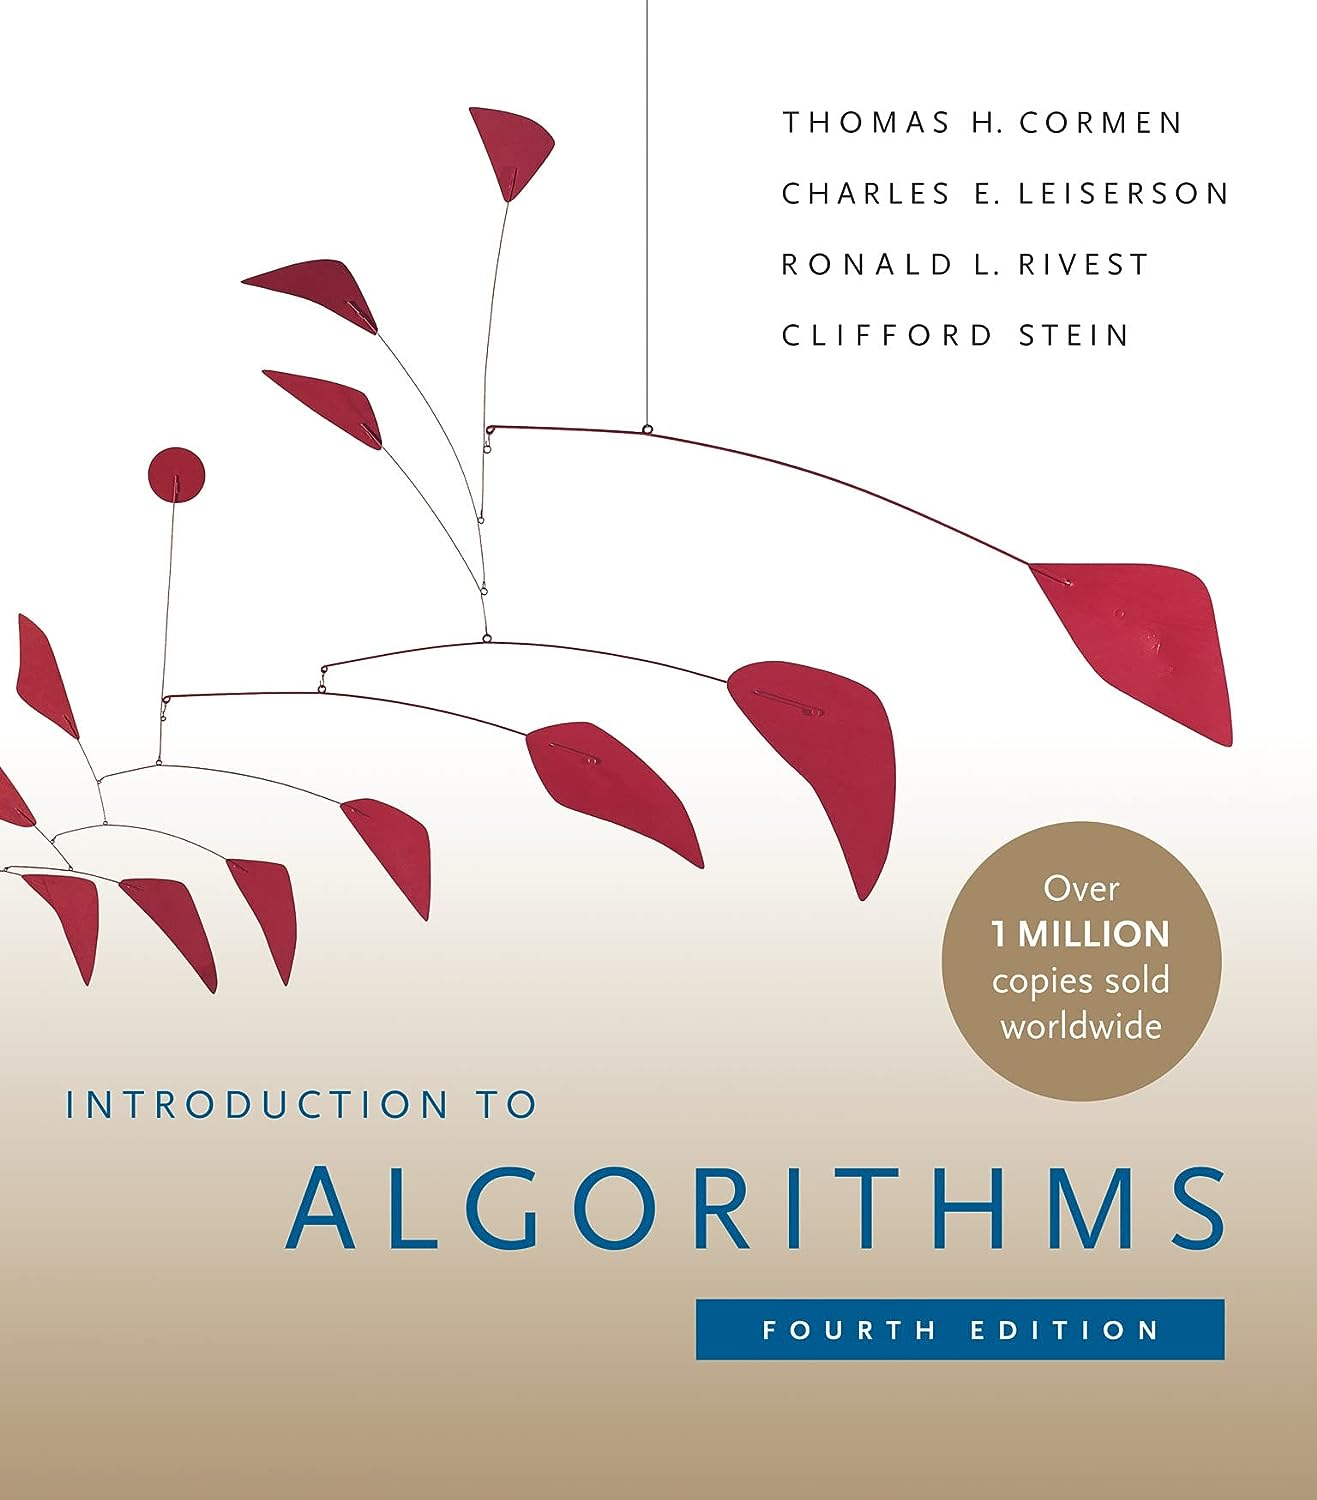
\includegraphics[width=0.24\textwidth]{cormen_4_cover}} 
    \label{fig:foobar}
\end{figure}
\end{frame}


%%%%%%%%%%%%%%%%%%%%%%%%%%%%%%%%%%%%%%%%%%%%%%%%%%%%%%%%%%%%%%%%%%%%%%%%%%%%%%%%%%%%%%%%%%%%%%%%%%
\begin{frame}[c]
%\frametitle{A first slide}

\begin{center}
\Huge Лекция 0.

\Huge Алгоритмы, вычислительные машины и программы
\end{center}

\end{frame}


%%%%%%%%%%%%%%%%%%%%%%%%%%%%%%%%%%%%%%%%%%%%%%%%%%%%%%%%%%%%%%%%%%%%%%%%%%%%%%%%%%%%%%%%%%%%%%%%%%
\begin{frame}
\frametitle{Алгоритмы, вычислительные машины и программы}
\framesubtitle{План лекции}

\begin{enumerate}
  \setcounter{enumi}{-1}
  \item{План лекции}
  \item{\textcolor{blue}{Понятие алгоритма}}
  \item{Вычислительные машины}
  \item{Алгоритмы и программы}
  \item{Алгоритмы и данные}
  \item{Битовые операции}

\end{enumerate}
\end{frame}

%%%%%%%%%%%%%%%%%%%%%%%%%%%%%%%%%%%%%%%%%%%%%%%%%%%%%%%%%%%%%%%%%%%%%%%%%%%%%%%%%%%%%%%%%%%%%%%%%%
\begin{frame}
\frametitle{Понятие алгоритма}
\framesubtitle{Неформальное понятие алгоритма}
\justifying
В повседневной жизни мы можем рассматривать \textcolor{red}{алгоритм} как последовательность действий, направленную на достижение желаемого результата.\newline

Алгоритмы для приготовления пищи называются рецепты.
Они включают заданный набор ингридиентов (\textcolor{red}{входных данных}), чётко определенную последовательность действий (\textcolor{red}{инструкции/команды}) и результат - блюдо с желаемым внешним видом и вкусовыми качествами.\newline

Для составления алгоритмов воспроизведения музыки используются ноты. Таким образом, человек может пошагово воспроизвести записанное и получить в качестве результата желаемую музыку.

\end{frame}

%%%%%%%%%%%%%%%%%%%%%%%%%%%%%%%%%%%%%%%%%%%%%%%%%%%%%%%%%%%%%%%%%%%%%%%%%%%%%%%%%%%%%%%%%%%%%%%%%%
\begin{frame}
\frametitle{Понятие алгоритма}
\framesubtitle{Более формальное понятие алгоритма}
\justifying
\textcolor{red} {Алгоритм} - понятная и точная последовательность шагов (вычислительная процедура), которая получает некоторое значение или набор значений (входные данные) и за конечное время выдает некоторое значение или набор значений в качестве результата (выходные данные). \newline\newline
Таким образом, алгоритм трансформирует входные данные в ответ.\newline

\textcolor{red} {Алгоритм} - фундаментальная концепция всей области компьютерных наук.\newline

В сфере информационных технологий нам будут интересны алгоритмы, которые способны решать \textcolor{red}{вычислительные задачи}, а исполнителями а этом случае будут являться \textcolor{red}{вычислительные машины}.

\end{frame}

%%%%%%%%%%%%%%%%%%%%%%%%%%%%%%%%%%%%%%%%%%%%%%%%%%%%%%%%%%%%%%%%%%%%%%%%%%%%%%%%%%%%%%%%%%%%%%%%%%
\begin{frame}
\frametitle{Алгоритмы, вычислительные машины и программы}
\framesubtitle{План лекции}

\begin{enumerate}
  \setcounter{enumi}{-1}
  \item{План лекции}
  \item{Понятие алгоритма}
  \item{\textcolor{blue}{Вычислительные машины}}
  \item{Алгоритмы и программы}
  \item{Алгоритмы и данные}
  \item{Битовые операции}

\end{enumerate}
\end{frame}

%%%%%%%%%%%%%%%%%%%%%%%%%%%%%%%%%%%%%%%%%%%%%%%%%%%%%%%%%%%%%%%%%%%%%%%%%%%%%%%%%%%%%%%%%%%%%%%%%
\begin{frame}
\frametitle{Вычислительные машины}
\framesubtitle{Алгоритмы и вычислительные машины}

Создание алгоритма для решения некоторой вычислительной задачи - важная работа. \newline \newline Как только правильный (с точки зрения выдаваемых результатов) и эффективный (с точки зрения затрачиваемых ресурсов) алгоритм придуман, решение рассматриваемой задачи больше не требует понимания принципов, на которых построен алгоритм. Далее все сводится лишь к последовательному исполнению шагов алгоритма.\newline

Чтобы автоматически выполнять уже имеющиеся эффективные алгоритмы, люди в течение нескольких столетий изобретали и улучшали \textcolor{red}{вычислительные машины}.


\end{frame}

%%%%%%%%%%%%%%%%%%%%%%%%%%%%%%%%%%%%%%%%%%%%%%%%%%%%%%%%%%%%%%%%%%%%%%%%%%%%%%%%%%%%%%%%%%%%%%%%%
\begin{frame}
\frametitle{Вычислительные машины}
\framesubtitle{Ранние вычислительные машины}
\justifying
Абак - одно из самых ранних устройств для выполнения арифметических операций. В большей степени являлось средством хранения и представления чисел, процесс вычислений проводился человеком. \newline

Первое запатентованное счетное устройство - механический калькулятор, созданный в 1640х годах Блезом Паскалем.
Состояло из спиц и колёсиков, умело складывать и вычитать.

\begin{figure}

    \captionsetup[subfigure]{labelformat=empty}
    \centering
    \subfigure[{\scriptsize \quad Abacus (Абак/Счёты)}]{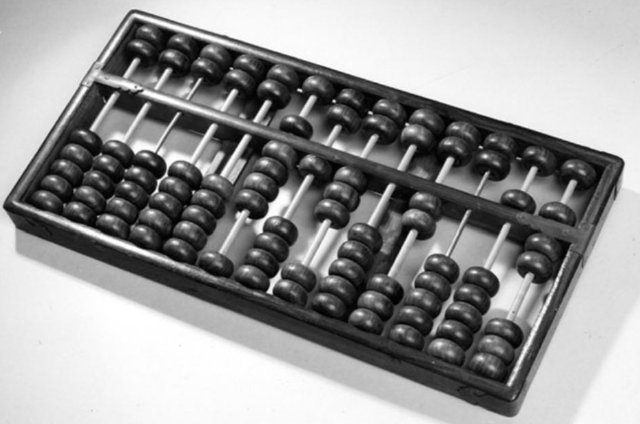
\includegraphics[width=0.32\textwidth]{abacus}} 
    \subfigure[{\newline \quad Калькулятор Паскаля}]{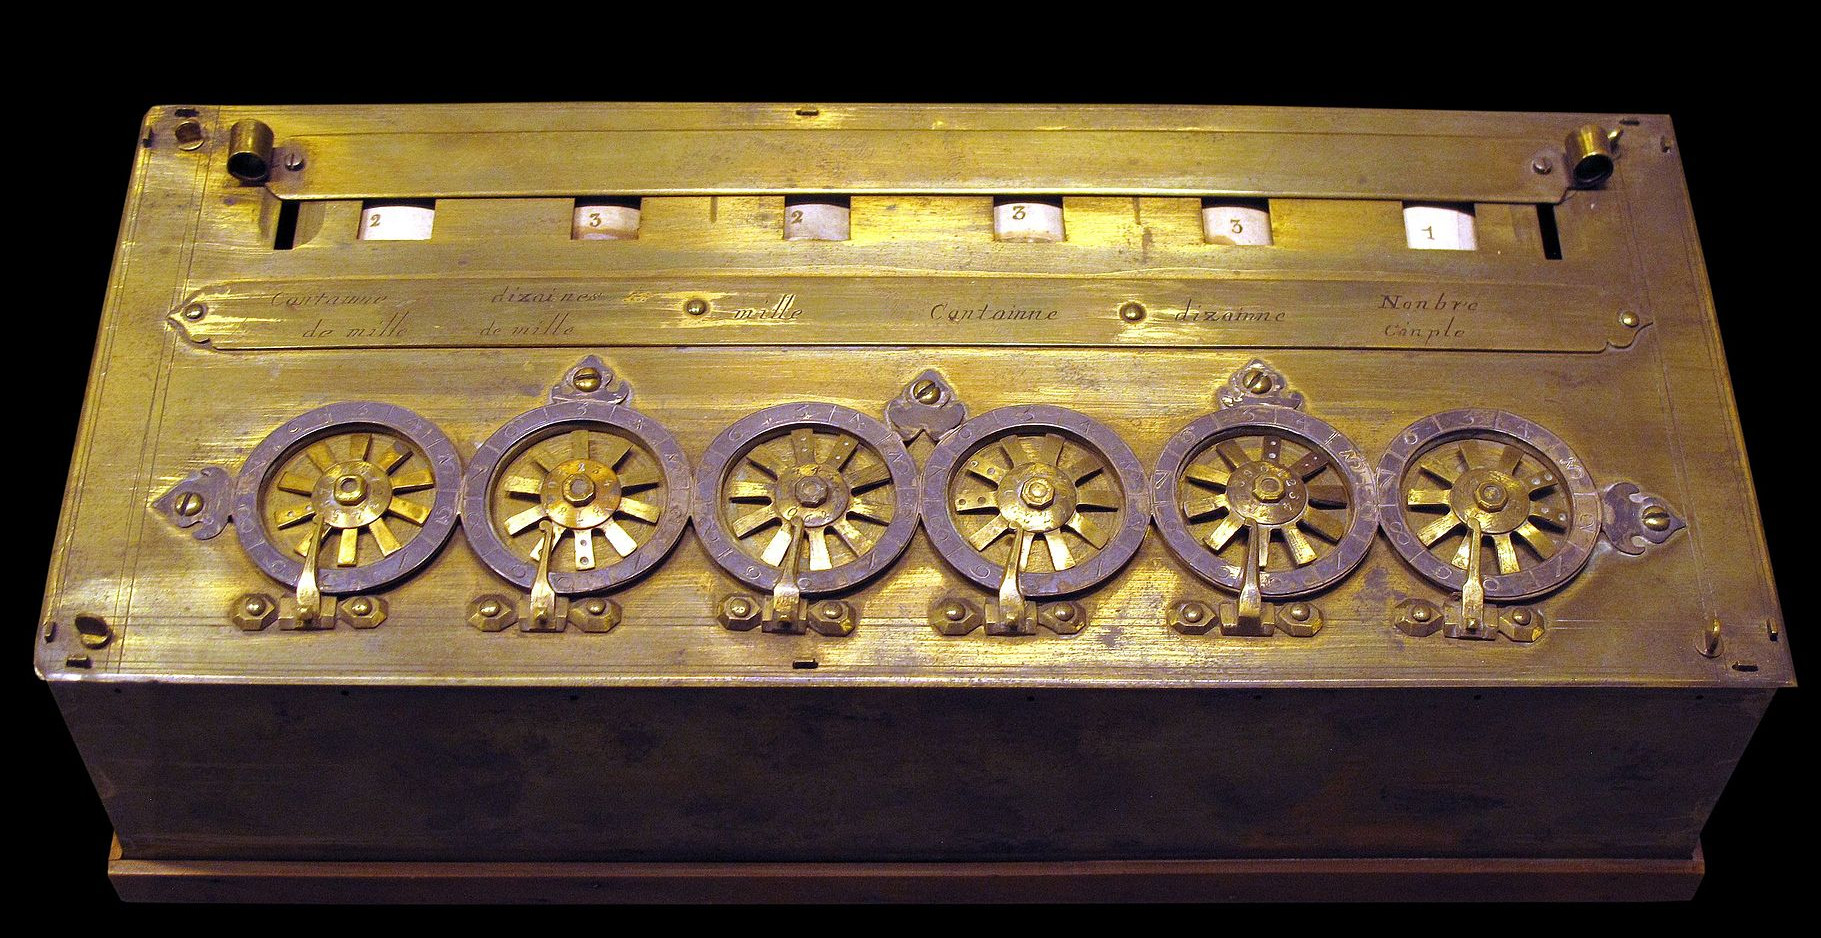
\includegraphics[width=0.41\textwidth]{pascal_calc}} 
\end{figure}

\end{frame}


%%%%%%%%%%%%%%%%%%%%%%%%%%%%%%%%%%%%%%%%%%%%%%%%%%%%%%%%%%%%%%%%%%%%%%%%%%%%%%%%%%%%%%%%%%%%%%%%%
\begin{frame}
\frametitle{Вычислительные машины}
\framesubtitle{Изобретения Чарльза Бэббиджа}
\begin{block}{}
\begin{columns}[]
\column{\dimexpr\linewidth-30mm}
\justifying
Позже английский математик и инженер Чарльз Бэббидж (1791 - 1871) создал \textcolor{red}{разностную машину (differential engine)}, способную вычислять синусы, косинусы, тангенсы и логарифмы. Вычисление этих функций разбивалось на элементарные арфиметические операции.\newline\newline
Далее в 1834 Бэббидж разработал проект счётной машины \textcolor{red}{общего назначения}, которая могла выполнять множество операций по инструкциям, задаваемых ей программным образом. \newline

Изобретение было названо \textcolor{red}{аналитической машиной (analytical engine)}. В проекте были собраны все инновации из других областей того времени.

\column{30mm}

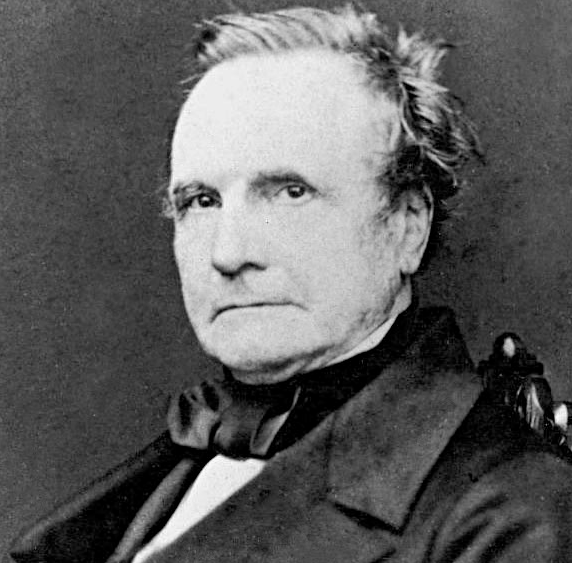
\includegraphics[width=30mm, height=25mm]{babbage}
\tiny Чарльз Бэббидж (Cambridge, UK), \href{https://en.wikipedia.org/wiki/Charles_Babbage}{Источник - Wikipedia} 
\newline\newline
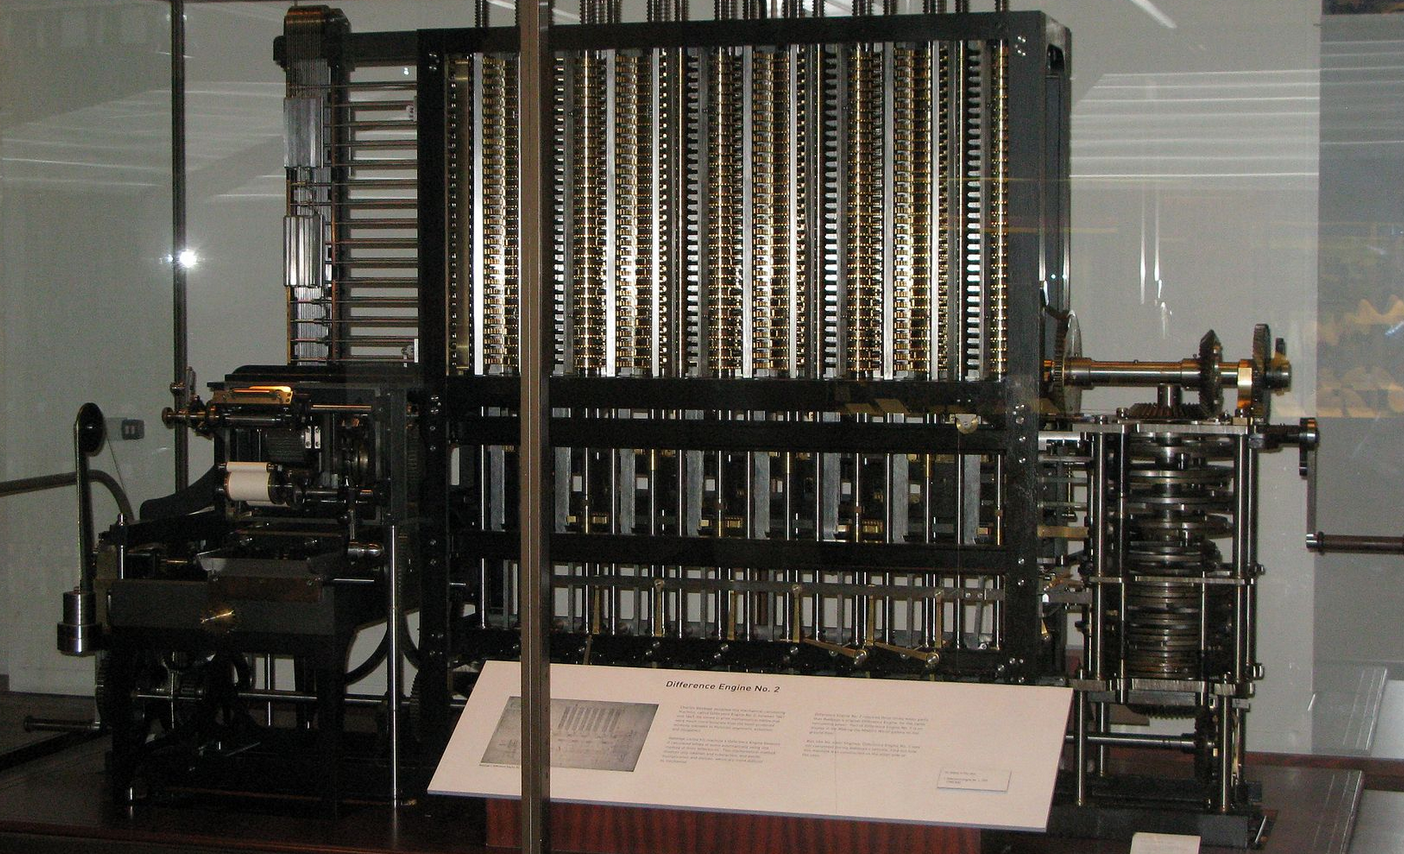
\includegraphics[width=30mm, height=25mm]{differential_engine}\newline
\tiny Разностная машина, \href{https://en.wikipedia.org/wiki/Charles_Babbage}{Источник - Wikipedia} 

\end{columns}
\end{block}
\end{frame}

%%%%%%%%%%%%%%%%%%%%%%%%%%%%%%%%%%%%%%%%%%%%%%%%%%%%%%%%%%%%%%%%%%%%%%%%%%%%%%%%%%%%%%%%%%%%%%%%%
\begin{frame}
\frametitle{Вычислительные машины}
\framesubtitle{Ада Августа Лавлейс (Байрон)}
\begin{block}{}
\begin{columns}[]
\column{\dimexpr\linewidth-30mm}
\justifying
Бэббидж выступил на съезде учёных в Турине. Луиджи Менабреа законспектировал его доклад, и опубликовал описание аналитической машины на французском языке.\newline\newline
\textcolor{red}{Ада Байрон} перевела эту статью на английский. Бэббидж был удивлён тем, как она разобралась в материале и предложил ей сделать примечания к переводу.\newline\newline
Примечания Ады Байрон по объему вдвое привысили оригинальную статью, эта работа стала первой опубликованной компьютерной программой, а Ада Байрон вошла в историю как первый программист. 

\column{30mm}

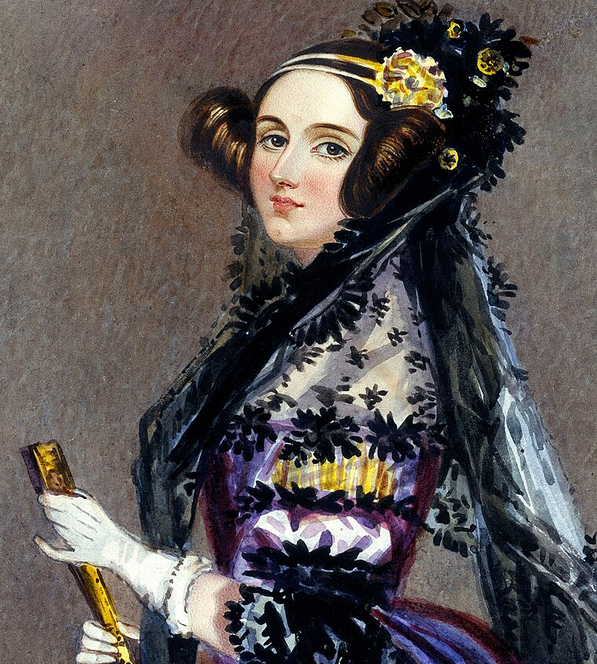
\includegraphics[width=30mm, height=40mm]{ada_byron}
\tiny Ада Августа Лавлейс (Байрон), \href{https://en.wikipedia.org/wiki/Ada_Lovelace}{Источник - Wikipedia} 
\end{columns}
\end{block}
\end{frame}

%%%%%%%%%%%%%%%%%%%%%%%%%%%%%%%%%%%%%%%%%%%%%%%%%%%%%%%%%%%%%%%%%%%%%%%%%%%%%%%%%%%%%%%%%%%%%%%%%
\begin{frame}
\frametitle{Вычислительные машины}
\framesubtitle{Ада Августа Лавлейс (Байрон)}
\justifying
Ада Лавлейс предложила несколько концепций, которые на многие годы опередили развитие вычислительное техники:
\begin{itemize}
\item{\textcolor{red}{Машина общего назначения} - запрограммирована для выполнения бесконечного числа и неограниченного круга задач}
\item{Функции машины не должны быть ограничены математикой и числами (например, работа со словами и символами)}
\item{Идея \textcolor{red}{подпрограмм}}
\item{\textcolor{red}{Искуственный интеллект}. "Аналитическая машина не претендует на создание чего-то своего. Она может выполнить любую команду, которую мы сумеем задать, но от нее нельзя ожидать вывода каких-либо аналитических соотношений или законов"}
\end{itemize}
\end{frame}

%%%%%%%%%%%%%%%%%%%%%%%%%%%%%%%%%%%%%%%%%%%%%%%%%%%%%%%%%%%%%%%%%%%%%%%%%%%%%%%%%%%%%%%%%%%%%%%%%
\begin{frame}
\frametitle{Вычислительные машины}
\framesubtitle{Электронные машины}
\justifying
\scriptsize
Технологии 19 века не позволяли создать многие из вышеперечисленных вариантов вычислительных машин относительно дешево. Но, с развитием электроники в первой половине 20 века эта проблема была решена.
Повсеместно, во всем мире стали появляться более совершенные вычислительные электронно-механические устройства.
\begin{itemize}
\item{\textcolor{red}{Модель К, 1940 год, Р.Штиблиц, Bell Labs} - электромеханические реле, не была полностью электронной. Не была универсальной, программируемой, предназначалась для определенной задачи.}

\item{\textcolor{red}{Z3, Г.Цузе, 1941} - первая автоматически контролируемое, программируемое электрическое двоичное устройство. Но не была полностью электронной, также были переключатели - щёлкающие реле. Не пошла в производство, была разрушена после бомбардировок Берлина в 1943.}

\item{\textcolor{red}{Компьютер Д.В.Атанасова} - Был первым электронным компьютером в мире (использовал электронные лампы). Но блоки памяти содержали механические вращающиеся барабаны. Не был программируемым и универсальным - был создан для решения систем линейных уравнений.
}

\item{\textcolor{red}{Машина Colossus I} - создана Максом Ньюманом, Томми Флауэрсом и Аланом Тьюрингом. Электронный, программируемый и работающий. Но не являлся компьютером общего назначения и тьюринг-полной машиной и также был узкоспециализированным - для взлома военных кодов Германии.}

\item{\textcolor{red}{Mark I Говарда Айкена} - Построенный с участием IBM и введенный в эксплуатацию в мае 1944 года бы программируемым, но электро-механическим, а не электронным.}

\end{itemize}
\end{frame}

%%%%%%%%%%%%%%%%%%%%%%%%%%%%%%%%%%%%%%%%%%%%%%%%%%%%%%%%%%%%%%%%%%%%%%%%%%%%%%%%%%%%%%%%%%%%%%%%%
\begin{frame}
\frametitle{Вычислительные машины}
\framesubtitle{ENIAC - первый компьютер}
\justifying
\textcolor{red}{ENIAC}, построенный \textcolor{red}{Джоном Мокли} и \textcolor{red}{Преспером Эккертом} в ноябре 1945 года был первой машиной, включающей все черты современного компьютера.

\begin{itemize}
\item{Полностью электронный (основанным на электронных лампах), быстрый}
\item{Программируемый}
\item{Компьютер общего назначения(теоретически мог решить любую задачу)}
\end{itemize}

\begin{figure}

    \captionsetup[subfigure]{labelformat=empty}
    \centering
    \subfigure[{\scriptsize \quad Команда программистов ENIAC}]{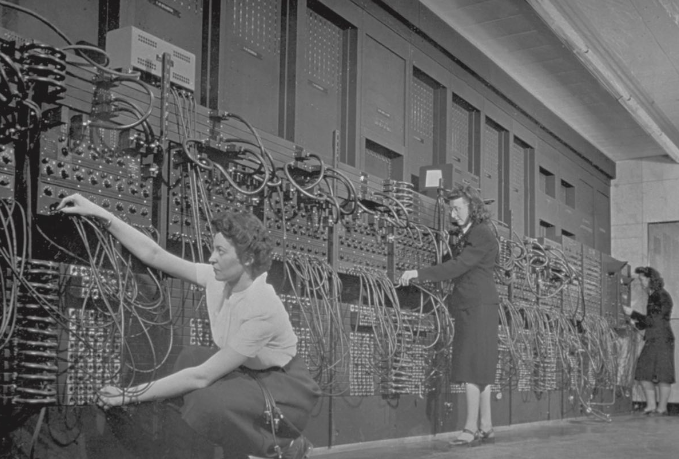
\includegraphics[width=0.4\textwidth]{women_eniac}} 
    \subfigure[{\newline \quad ENIAC}]{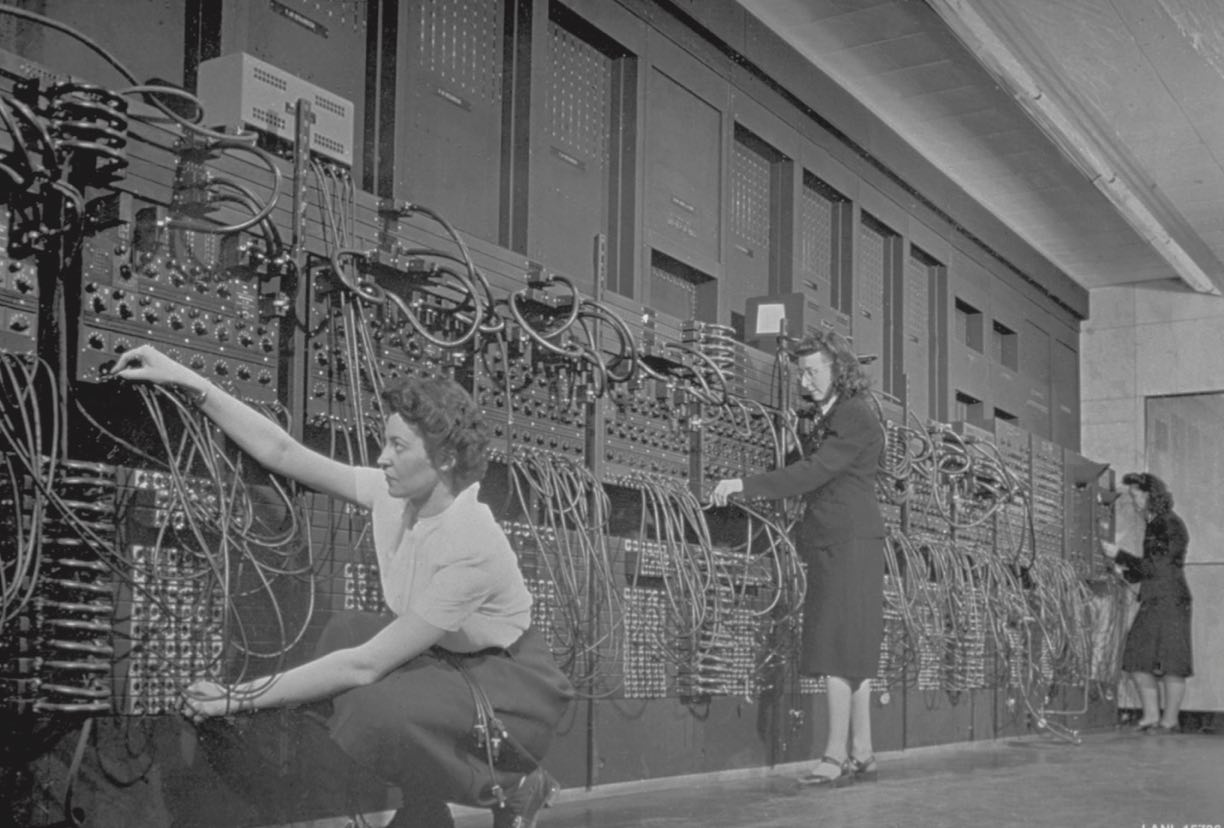
\includegraphics[width=0.41\textwidth]{eniac}} 
\end{figure}
\end{frame}

%%%%%%%%%%%%%%%%%%%%%%%%%%%%%%%%%%%%%%%%%%%%%%%%%%%%%%%%%%%%%%%%%%%%%%%%%%%%%%%%%%%%%%%%%%%%%%%%%
\begin{frame}
\frametitle{Вычислительные машины}
\framesubtitle{Транзистор}
\justifying

Электронные лампы были дорогими, громоздкими, поглощали много энергии. \newline Для компьютеров того времени их было необходимо очень много.\newline\newline
Наиболее значимым в этот период являлось изобретение \textcolor{red}{транзисторов}. \newline За это, команда Bell Labs в лице \textcolor{red}{Уиллиама Шокли,  Джон Бардина} и \textcolor{red}{Уолтера Браттейна} была удостоена Нобелевской премии по физике.

\begin{figure}
    \captionsetup[subfigure]{labelformat=empty}
    \centering
    \subfigure[{ \scriptsize \quad Д.Бардин, У.Шокли, У.Браттейн}]{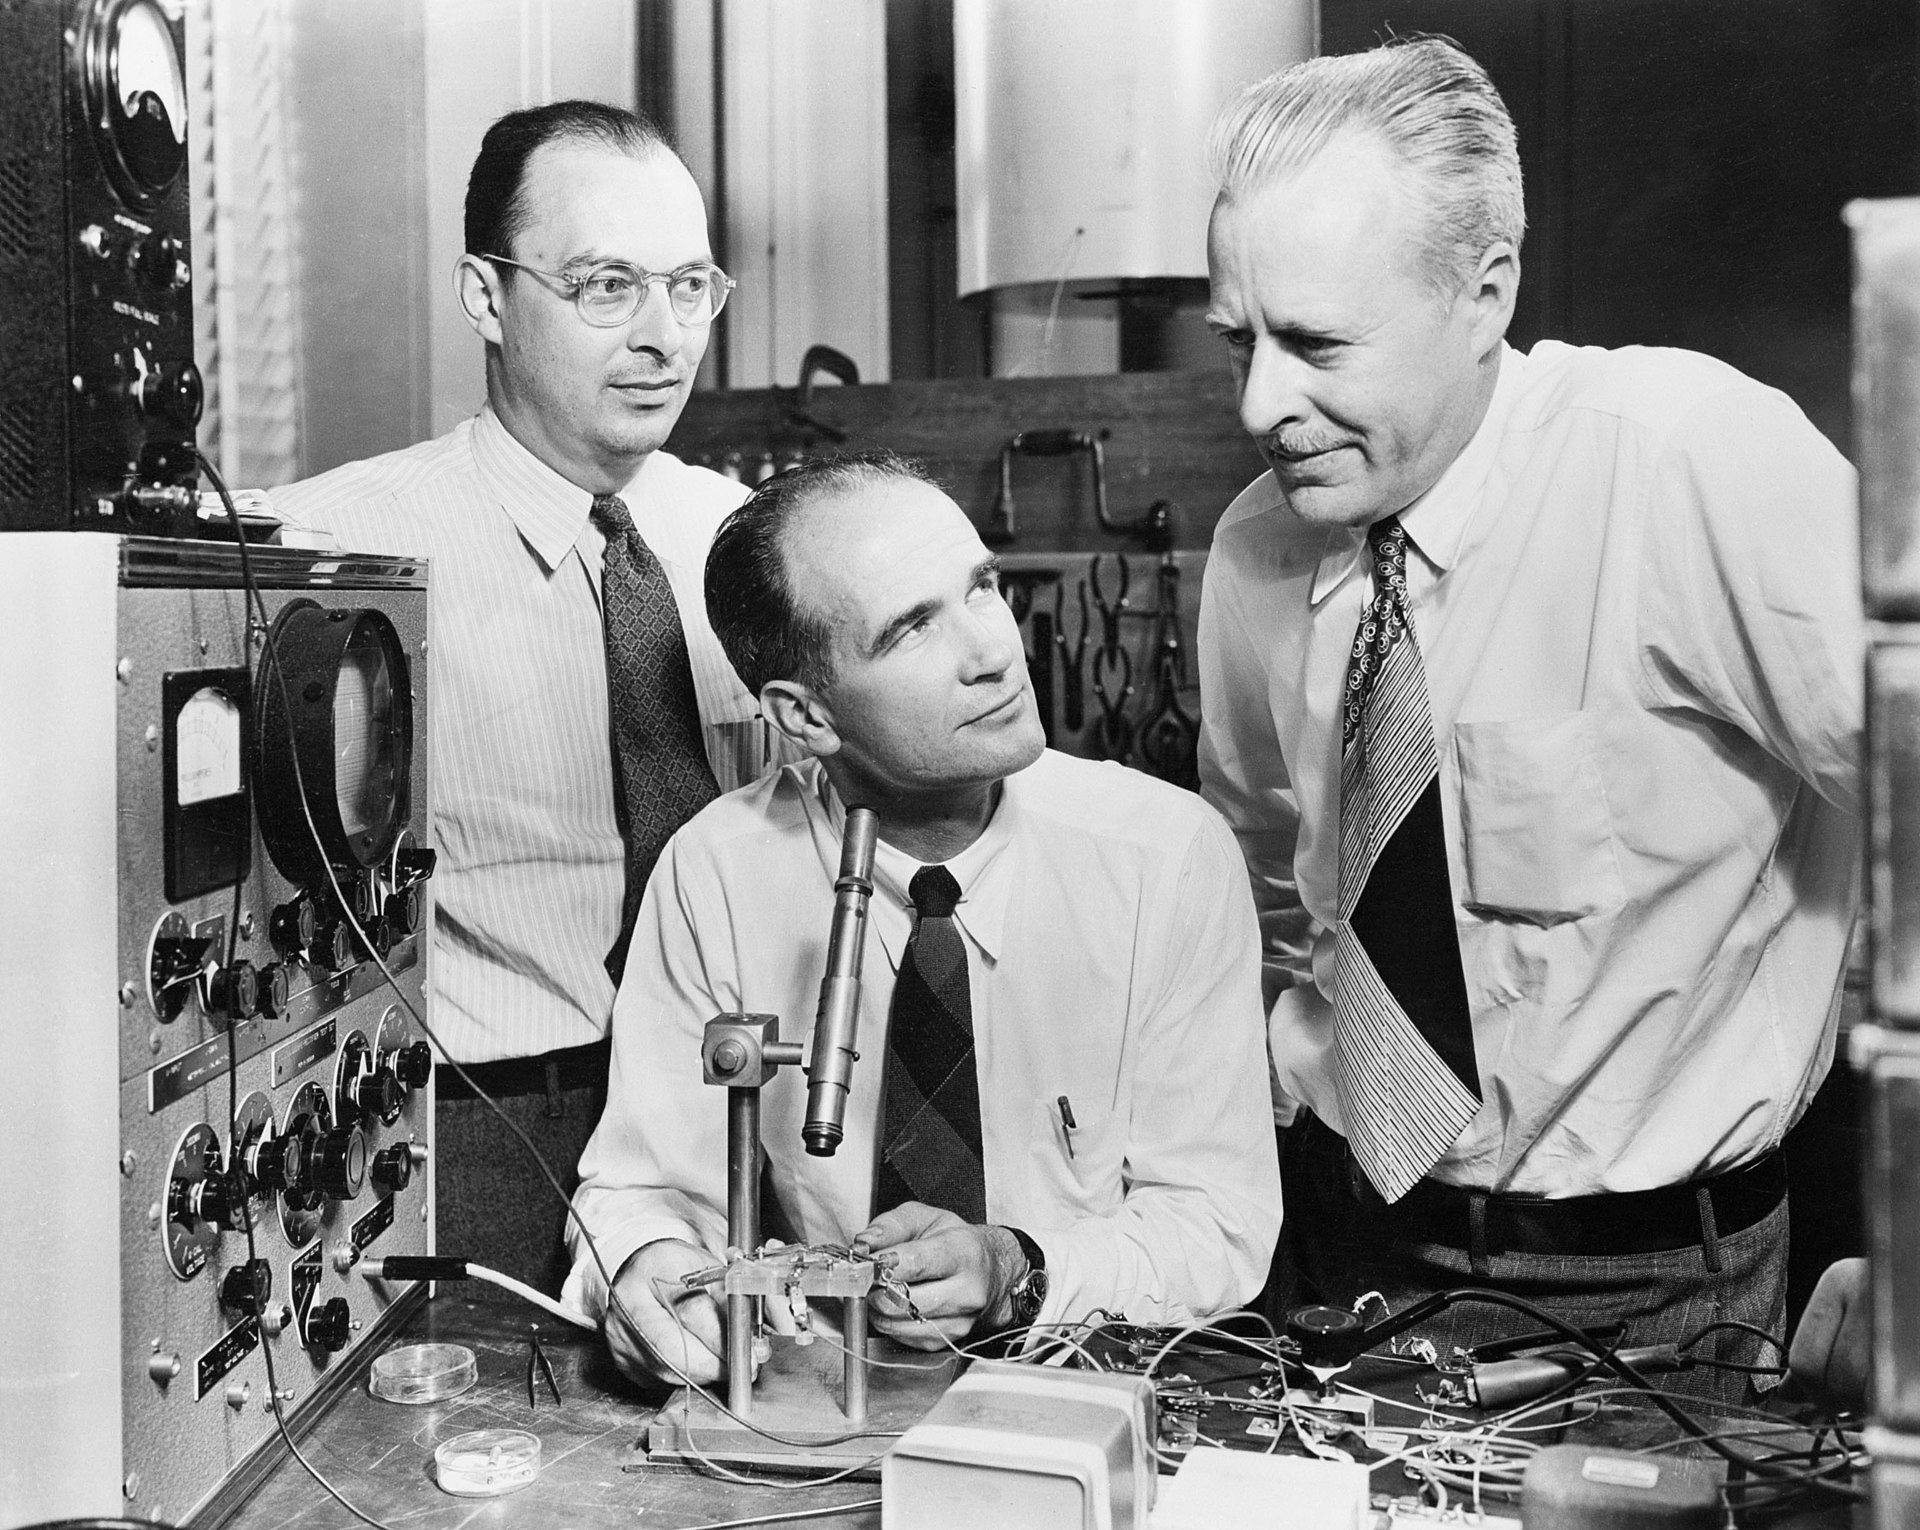
\includegraphics[width=60mm, height=35mm]{transistor_team}} 
\end{figure}
\end{frame}

%%%%%%%%%%%%%%%%%%%%%%%%%%%%%%%%%%%%%%%%%%%%%%%%%%%%%%%%%%%%%%%%%%%%%%%%%%%%%%%%%%%%%%%%%%%%%%%%%
\begin{frame}
\frametitle{Вычислительные машины}
\framesubtitle{Микрочип}
\justifying
\small
В \textcolor{red}{Texas Instruments (Джон Килби}) и \textcolor{red}{Fairchild Semiconductors (Роберт Нойс и Гордон Мур)} был изобретен \textcolor{red}{микрочип}. Идея - помеcтить транзисторы и другие элементы на единую кремниевую пластину. Вместо связующих их проволочек было предложено пропечатать небольшие медные линии. В 2000 году за это открытие присуждена Нобелевская премия.\newline\newline 
Производство таких схем стало надежным, массовым и дешевым. В результате, машины размером с комнату 1940-е годы были уменьшены за десятилетия до размеров одиночных шкафов. Вычислительная мощность машин стала удваиваться каждые два года.

\begin{figure}
    \captionsetup[subfigure]{labelformat=empty}
    \centering
    %%\subfigure[{ \scriptsize \quad Д.Бардин, У.Шокли, У.Браттейн}]{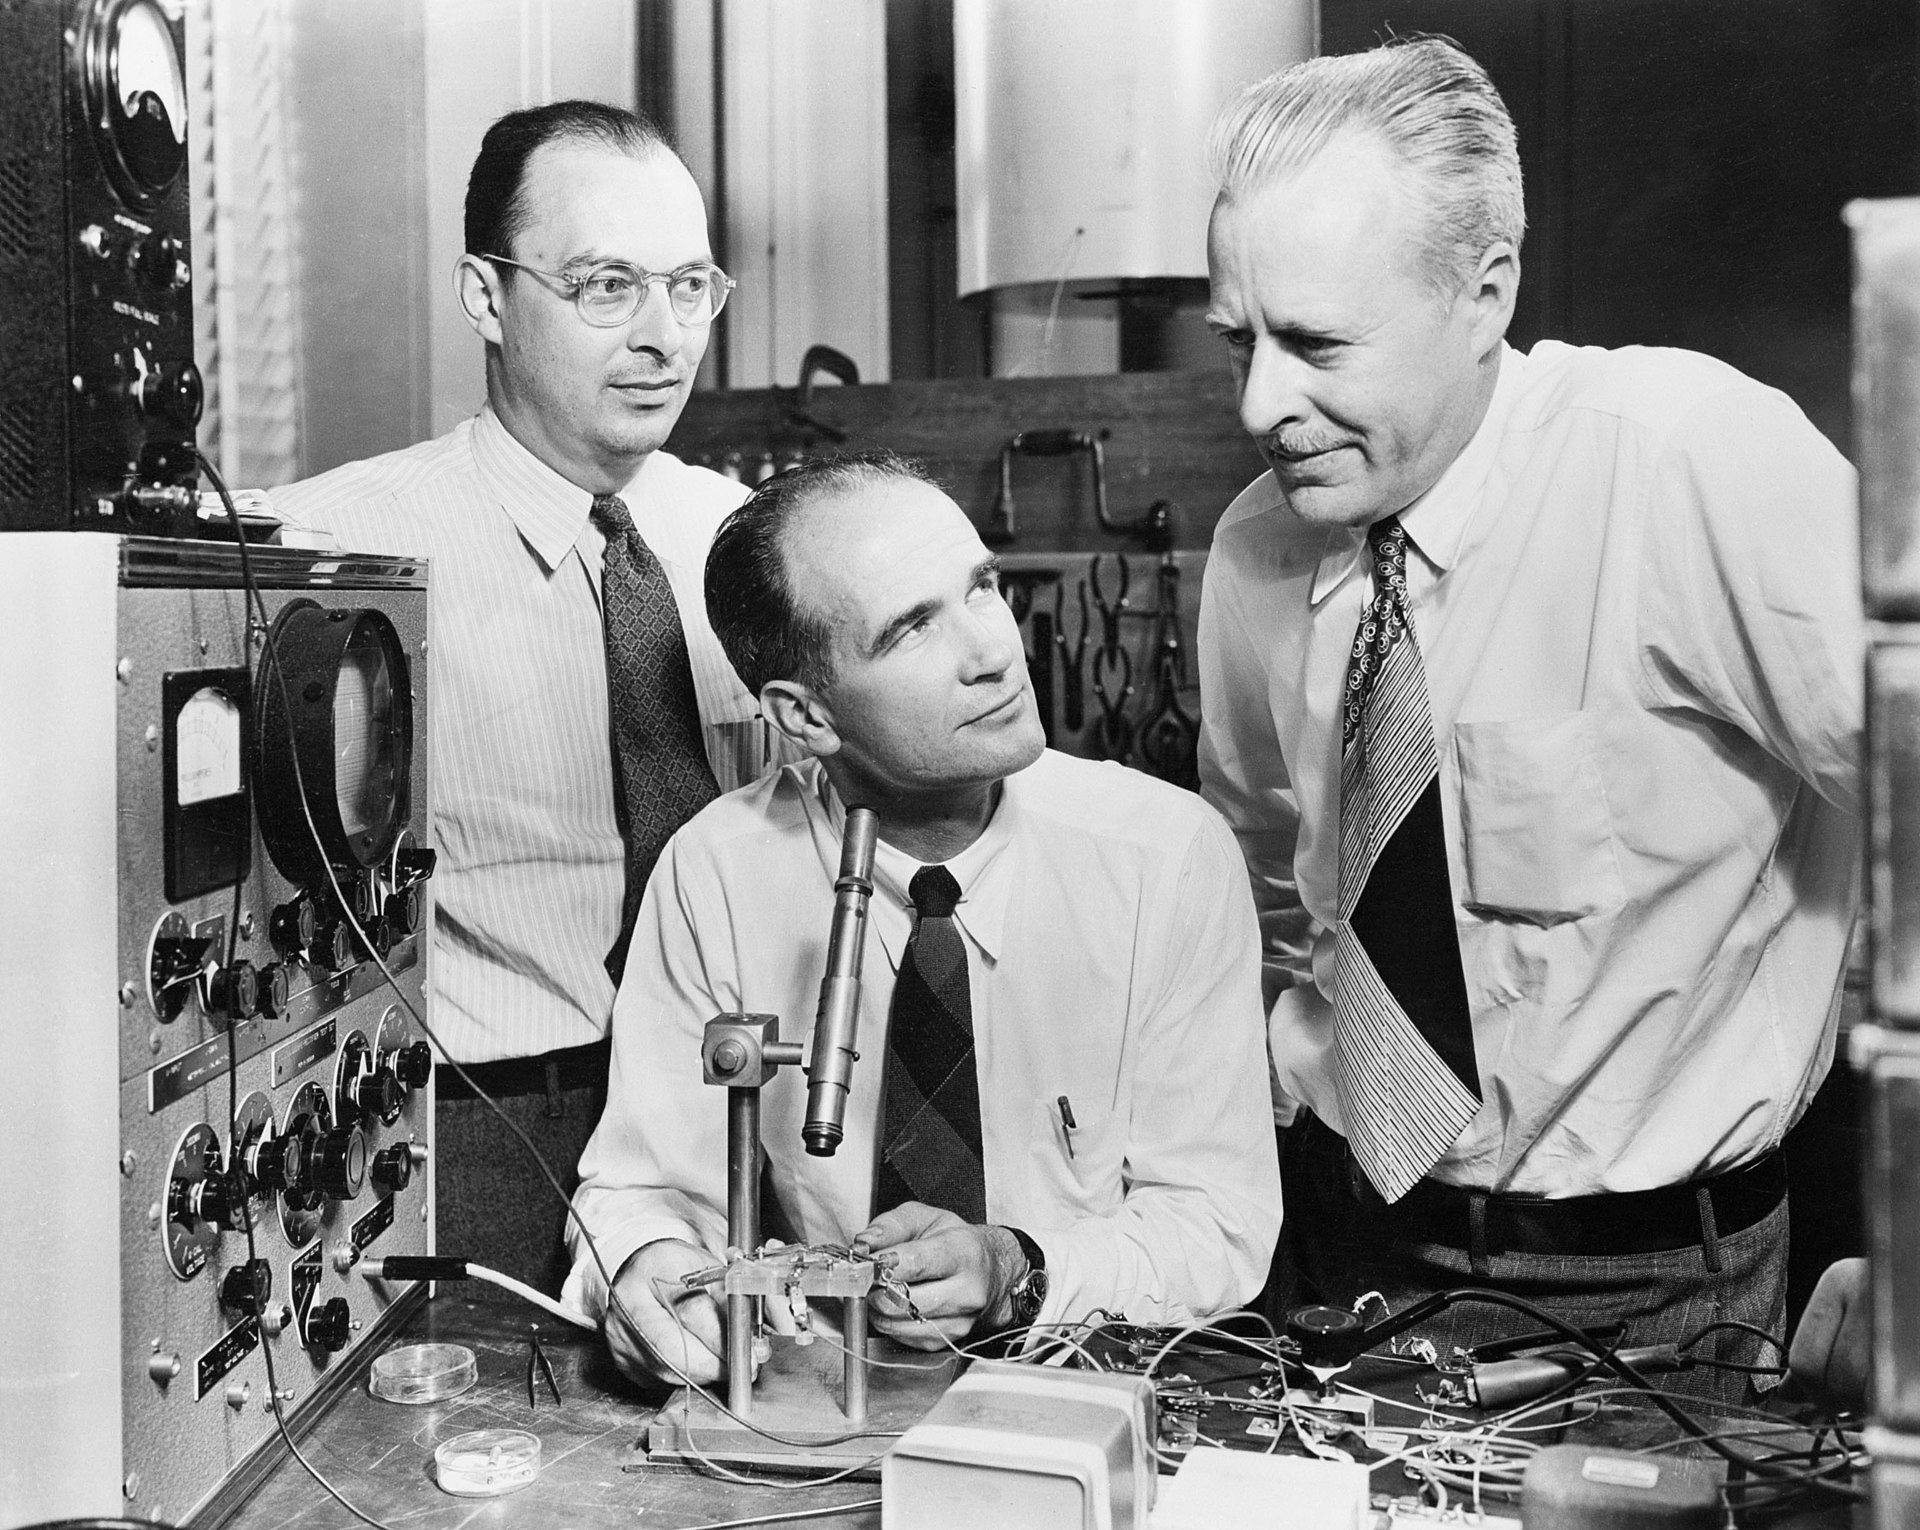
\includegraphics[width=60mm, height=35mm]{transistor_team}} 
\end{figure}
\end{frame}

%%%%%%%%%%%%%%%%%%%%%%%%%%%%%%%%%%%%%%%%%%%%%%%%%%%%%%%%%%%%%%%%%%%%%%%%%%%%%%%%%%%%%%%%%%%%%%%%%
\begin{frame}
\frametitle{Вычислительные машины}
\framesubtitle{Микрочип}
\justifying
\small

Количество транзисторов в современных процессорах исчисляется миллиардами.

\begin{figure}
    \captionsetup[subfigure]{labelformat=empty}
    \centering
    %%\subfigure[{ \scriptsize \quad Д.Бардин, У.Шокли, У.Браттейн}]{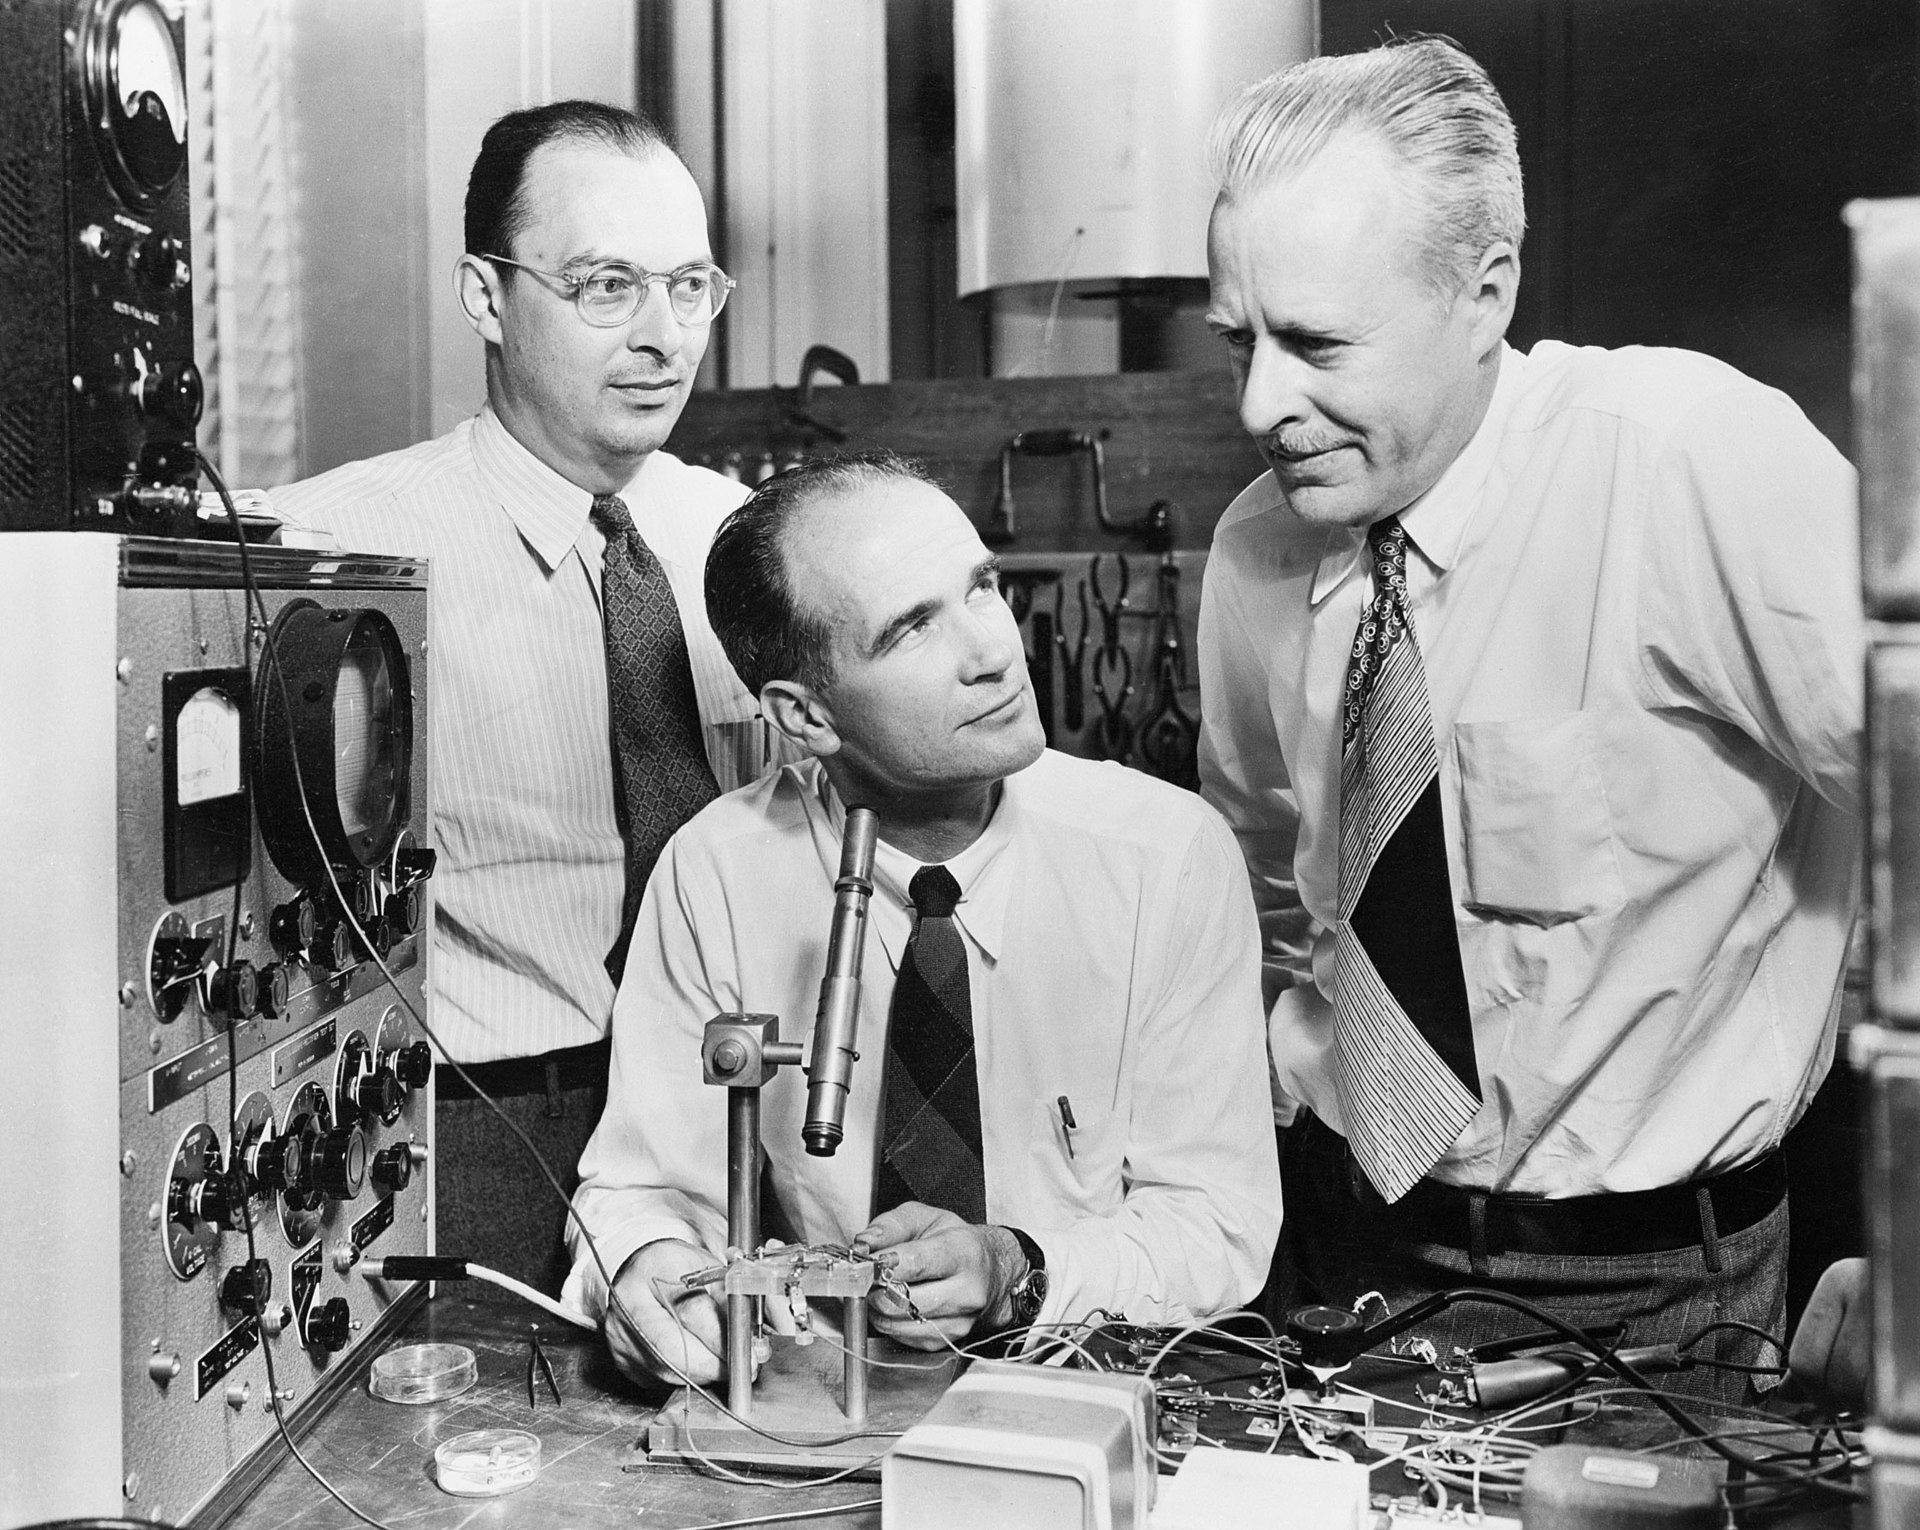
\includegraphics[width=60mm, height=35mm]{transistor_team}} 
\end{figure}
\end{frame}

%%%%%%%%%%%%%%%%%%%%%%%%%%%%%%%%%%%%%%%%%%%%%%%%%%%%%%%%%%%%%%%%%%%%%%%%%%%%%%%%%%%%%%%%%%%%%%%%%%
\begin{frame}
\frametitle{Алгоритмы, вычислительные машины и программы}
\framesubtitle{План лекции}

\begin{enumerate}
  \setcounter{enumi}{-1}
  \item{План лекции}
  \item{Понятие алгоритма}
  \item{Вычислительные машины}
  \item{\textcolor{blue}{Алгоритмы и программы}}
  \item{Алгоритмы и данные}
  \item{Битовые операции}

\end{enumerate}
\end{frame}


%%%%%%%%%%%%%%%%%%%%%%%%%%%%%%%%%%%%%%%%%%%%%%%%%%%%%%%%%%%%%%%%%%%%%%%%%%%%%%%%%%%%%%%%%%%%%%%%%%
\begin{frame}
\frametitle{Алгоритмы и программы}
\framesubtitle{Программы и двоичный код}
\justifying

Алгоритмы являются подробными и точными инструкциями по решению какой-либо задачи. Каждый алгоритм предназначается для некоторого исполнителя.\newline

 В реальной жизни исполнителями как правило являются люди или вычислительные машины. Например, инструкция по сборке мебели - это алгоритм предназначаемый для исполнителя-человека.\newline

Однако, самые сложные задачи, связанные с обработкой, хранением и передачей информации  человек умышленно поручил вычислительным машинам.
Вычислительные машины оперируют лишь двумя состояниями связанными с наличием тока или его отсутствием.\newline

Эта физическая сущность компьютеров заставила людей использовать двоичную систему счисления или \textcolor{red}{двоичный код}.

\end{frame}

%%%%%%%%%%%%%%%%%%%%%%%%%%%%%%%%%%%%%%%%%%%%%%%%%%%%%%%%%%%%%%%%%%%%%%%%%%%%%%%%%%%%%%%%%%%%%%%%%%
\begin{frame}
\frametitle{Алгоритмы и программы}
\framesubtitle{Программы и двоичный код}
\justifying

Люди формулируют алгоритмы на понятном им языке, а компьютеры на языке двоичной системы счисления - с помощью нулей и единиц.\newline\newline Для формализации и описания алгоритмов в более понятной для вычислительных машин манере были созданы \textcolor{red}{языки программирования}.\newline\newline 
Алгоритм решения задачи, записанный на конкретном языке программирования называется \textcolor{red}{программой}. То есть, программа это более узкое понятие, а алгоритм более широкое. Программа - это один из способов записи алгоритма. \newline\newline 
\textcolor{red}{Программа} – набор инструкций на специальном языке, которые могут быть выполнены компьютером.

\end{frame}

%%%%%%%%%%%%%%%%%%%%%%%%%%%%%%%%%%%%%%%%%%%%%%%%%%%%%%%%%%%%%%%%%%%%%%%%%%%%%%%%%%%%%%%%%%%%%%%%%%
\begin{frame}
\frametitle{Алгоритмы и программы}
\framesubtitle{Машинный язык}
\justifying
\small
Языки программирования можно условно разделить на несколько категорий.\newline\newline
\textcolor{red}{Машинный язык}

Программа на машинном языке читается компьютером напрямую, без промежуточных шагов.\newline

Программа в машинном коде состоит из последовательности машинных инструкций в двоичном коде, которые содержат коды операций и ячейки памяти, участвующие в операции.


\begin{figure}
    \captionsetup[subfigure]{labelformat=empty}
    \centering
    \subfigure[{ \scriptsize \quad Пример двоичного кода}]{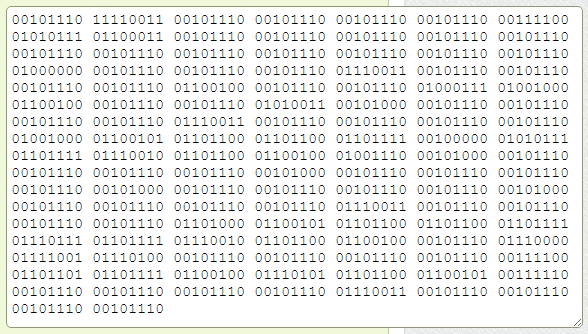
\includegraphics[width=40mm, height=20mm]{/home/llyy/Yandex.Disk/personal/knowledge/general/algorithms_course/repo/algorithms_course/0_intro/images/binary_hw}} 
    \subfigure[{ \scriptsize \quad Пример hex кода}]{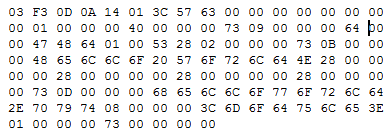
\includegraphics[width=40mm, height=20mm]{/home/llyy/Yandex.Disk/personal/knowledge/general/algorithms_course/repo/algorithms_course/0_intro/images/hex_hw}} 
    \subfigure[{ \scriptsize \quad Пример программиста на машинном языке}]{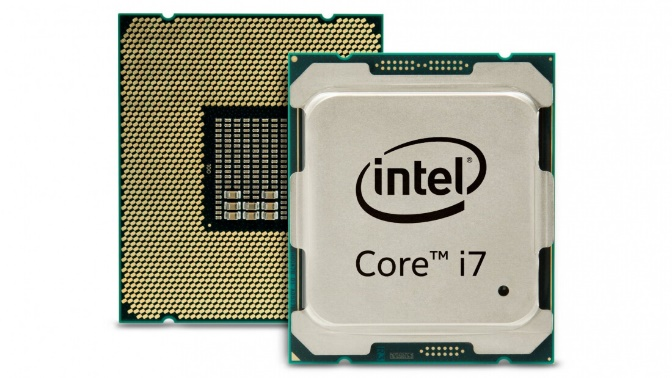
\includegraphics[width=40mm, height=20mm]{processor_unit}} 
\end{figure}
\end{frame}

%%%%%%%%%%%%%%%%%%%%%%%%%%%%%%%%%%%%%%%%%%%%%%%%%%%%%%%%%%%%%%%%%%%%%%%%%%%%%%%%%%%%%%%%%%%%%%%%%%
\begin{frame}
\frametitle{Алгоритмы и программы}
\framesubtitle{Ассемблер}
\justifying
\small

\textcolor{red}{Ассемблер (assembler)}

Символьное представление машинного языка конкретного процессора.\newline

Обычно каждая строка кода сборки производит одну машинную инструкцию.\newline

Программирование на ассемблере медленное и подвержено ошибкам, но более эффективно с точки зрения производительности оборудования.

\begin{figure}
    \captionsetup[subfigure]{labelformat=empty}
    \centering
    \subfigure[{ \scriptsize \quad Пример кода на ASM}]{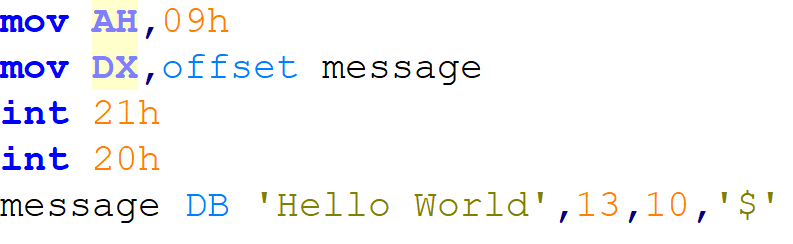
\includegraphics[width=70mm, height=25mm]{/home/llyy/Yandex.Disk/personal/knowledge/general/algorithms_course/repo/algorithms_course/0_intro/images/assembler_code_example}} 
    \subfigure[{ \scriptsize \quad Пример программиста на ASM}]{
\includegraphics[width=50mm, height=30mm]{old_geek}} 
\end{figure}
\end{frame}

%%%%%%%%%%%%%%%%%%%%%%%%%%%%%%%%%%%%%%%%%%%%%%%%%%%%%%%%%%%%%%%%%%%%%%%%%%%%%%%%%%%%%%%%%%%%%%%%%%
\begin{frame}
\frametitle{Алгоритмы и программы}
\framesubtitle{Языки программирования высокого уровня}
\justifying
\small

\textcolor{red}{Языки программирования высокого уровня (high-level programming languages)}\newline


Языки программирования, в котором используются операторы, состоящие из похожих на английские ключевых слов, таких как «FOR», «PRINT» или «IF».\newline

Каждое утверждение соответствует нескольким инструкциям машинного языка.\newline

\begin{figure}
    \captionsetup[subfigure]{labelformat=empty}
    \centering
    \subfigure[{ \scriptsize \quad Пример кода на Паскале (ЯВУ)}]{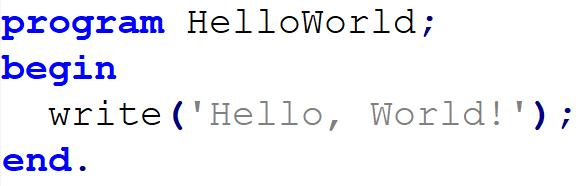
\includegraphics[width=65mm, height=25mm]{/home/llyy/Yandex.Disk/personal/knowledge/general/algorithms_course/repo/algorithms_course/0_intro/images/pascal_code_example}} 
    \subfigure[{ \scriptsize \quad Пример программиста на Паскале}]{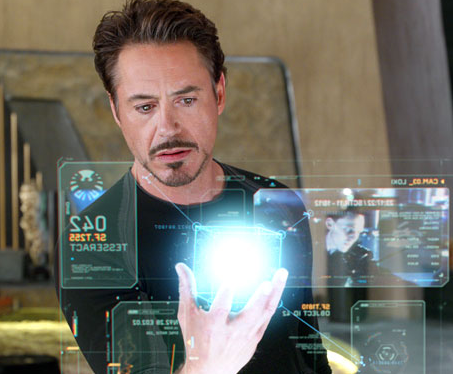
\includegraphics[width=50mm, height=30mm]{tony_start}} 
\end{figure}
\end{frame}

%%%%%%%%%%%%%%%%%%%%%%%%%%%%%%%%%%%%%%%%%%%%%%%%%%%%%%%%%%%%%%%%%%%%%%%%%%%%%%%%%%%%%%%%%%%%%%%%%%
\begin{frame}
\frametitle{Алгоритмы и программы}
\framesubtitle{Трансляция}
\justifying
\textcolor{red}{Транслятор} – программа, обеспечивающая перевод написанного нами исходного кода на внутренний язык компьютера. \newline\newline
Обычно выделяют трансляторы двух типов: \textcolor{red}{компилятор} и \textcolor{red}{интерпретатор}
\begin{figure}
    \captionsetup[subfigure]{labelformat=empty}
    \centering
    \subfigure[{ \scriptsize \quad Трансляция, \href{https://www.cs.mtsu.edu/~xyang/2170/computerLanguages.html}{Источник} }]{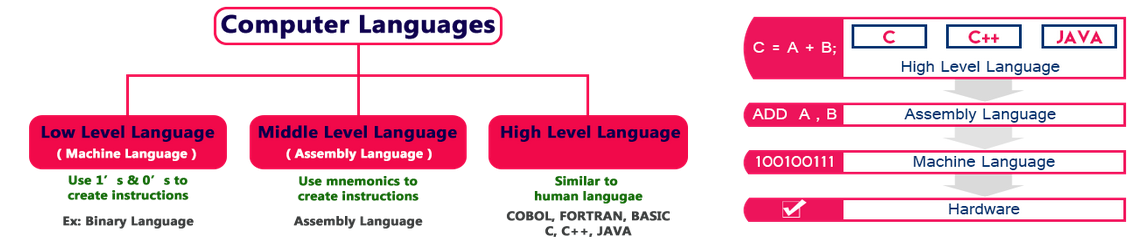
\includegraphics[width=120mm, height=30mm]{programming_translation}} 
\end{figure}
\end{frame}

%%%%%%%%%%%%%%%%%%%%%%%%%%%%%%%%%%%%%%%%%%%%%%%%%%%%%%%%%%%%%%%%%%%%%%%%%%%%%%%%%%%%%%%%%%%%%%%%%
\begin{frame}
\frametitle{Алгоритмы и программы}
\framesubtitle{Компиляция}
\begin{block}{}
\begin{columns}[]
\column{\dimexpr\linewidth-40mm}
\justifying
\small
\textcolor{red}{Компилятор} — это программа, которая преобразует исходный код, написанный на одном из языков программирования, в исполняемый машинный код или в промежуточный код (например, байт-код).\newline\newline
Компиляторы выполняют анализ и оптимизацию кода, чтобы создать эффективный и быстрый исполняемый файл.\newline

Основные функции компилятора:
\begin{itemize}
\item{проверка синтаксиса исходного кода}
\item{генерация машинного кода или байт-кода}
\item{оптимизация кода для повышения производительности}
\item{создание файлов объектного кода для компоновки с другими модулями}
\end{itemize}

\column{40mm}

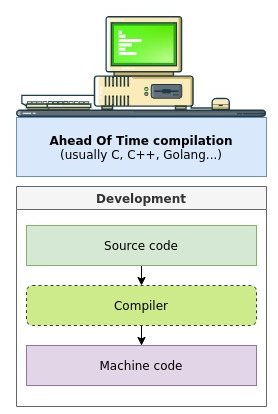
\includegraphics[width=40mm, height=60mm]{/home/llyy/Yandex.Disk/personal/knowledge/general/algorithms_course/repo/algorithms_course/0_intro/images/compiler_code_stage}
\centering
\tiny Компиляция, \href{https://ya.ru}{источник} 

\end{columns}
\end{block}
\end{frame}

%%%%%%%%%%%%%%%%%%%%%%%%%%%%%%%%%%%%%%%%%%%%%%%%%%%%%%%%%%%%%%%%%%%%%%%%%%%%%%%%%%%%%%%%%%%%%%%%%
\begin{frame}
\frametitle{Алгоритмы и программы}
\framesubtitle{Интерпретация}
\begin{block}{}
\begin{columns}[]
\column{\dimexpr\linewidth-40mm}
\justifying
\small
\textcolor{red}{Интерпретатор} — это программа, которая выполняет исходный код программы построчно. В отличие от компилятора, интерпретатор не переводит программу в машинный код, а сразу выполняет инструкции.\newline\newline
Основные функции интерпретатора:
\begin{itemize}
\item{чтение исходного кода программы}
\item{последовательное выполнение каждой строки кода}
\item{обработка ошибок и исключений во время выполнения программы}
\end{itemize}

Известные интерпретируемые языки программирования - Python, Java.

\column{40mm}

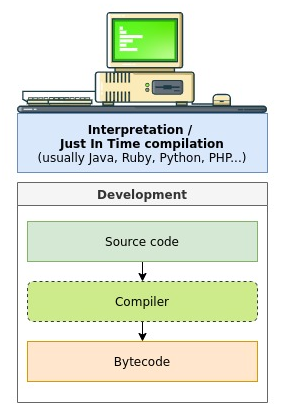
\includegraphics[width=40mm, height=60mm]{/home/llyy/Yandex.Disk/personal/knowledge/general/algorithms_course/repo/algorithms_course/0_intro/images/interpreter_code_stage}
\centering
\tiny Интерпретация, \href{https://ya.ru}{источник} 

\end{columns}
\end{block}
\end{frame}

%%%%%%%%%%%%%%%%%%%%%%%%%%%%%%%%%%%%%%%%%%%%%%%%%%%%%%%%%%%%%%%%%%%%%%%%%%%%%%%%%%%%%%%%%%%%%%%%%
\begin{frame}
\frametitle{Алгоритмы и программы}
\framesubtitle{Компиляция vs Интерпретация}
\justifying
\small
\centering
Компиляция vs Интерпретация в процессе выполнения кода

\begin{figure}
    \captionsetup[subfigure]{labelformat=empty}
    \centering
    \subfigure[{ \scriptsize \quad После компиляции}]{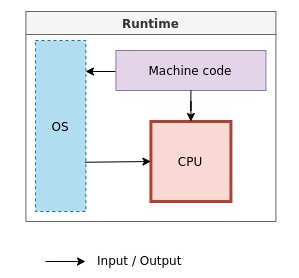
\includegraphics[width=55mm, height=55mm]{/home/llyy/Yandex.Disk/personal/knowledge/general/algorithms_course/repo/algorithms_course/0_intro/images/compiler_run_stage}} 
    \subfigure[{ \scriptsize \quad После интерпретации}]{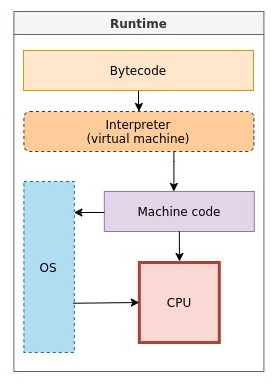
\includegraphics[width=50mm, height=55mm]{/home/llyy/Yandex.Disk/personal/knowledge/general/algorithms_course/repo/algorithms_course/0_intro/images/interpreter_run_stage}}
\end{figure}
\end{frame}

%%%%%%%%%%%%%%%%%%%%%%%%%%%%%%%%%%%%%%%%%%%%%%%%%%%%%%%%%%%%%%%%%%%%%%%%%%%%%%%%%%%%%%%%%%%%%%%%%
\begin{frame}
\frametitle{Алгоритмы и программы}
\framesubtitle{Трансляция исходного кода в машинный в C/C++}
\justifying
\small
\centering
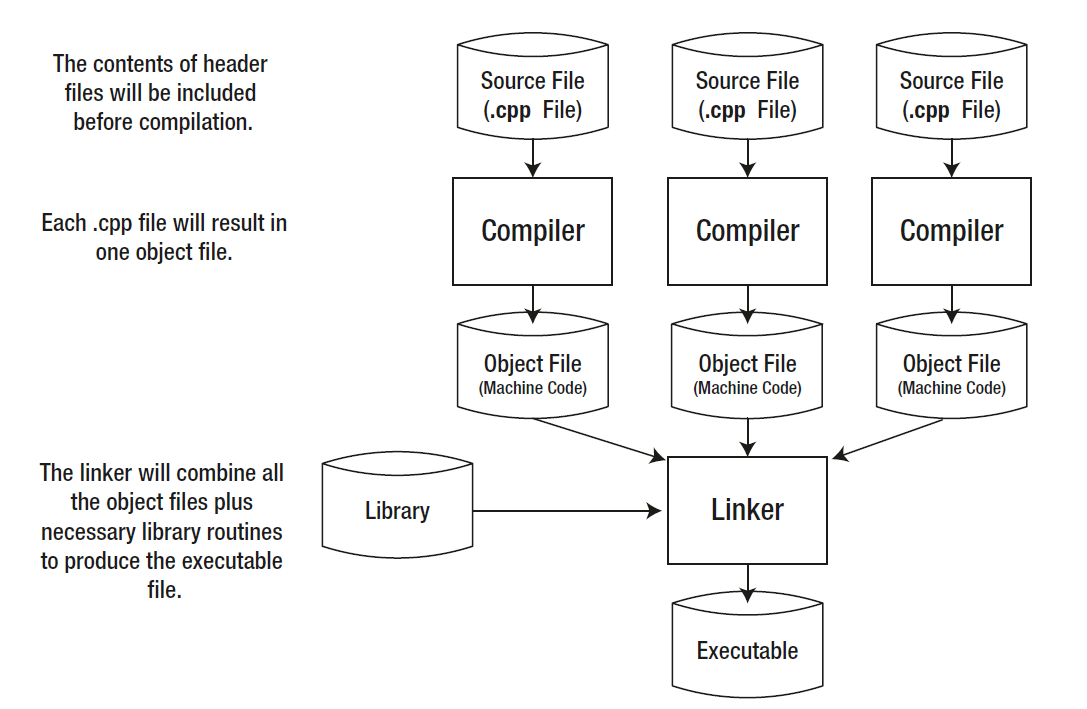
\includegraphics[width=90mm, height=60mm]{/home/llyy/Yandex.Disk/personal/knowledge/general/algorithms_course/repo/algorithms_course/0_intro/images/cpp_how_compile}

\scriptsize Источник - C++20 from novice to professional
\end{frame}

%%%%%%%%%%%%%%%%%%%%%%%%%%%%%%%%%%%%%%%%%%%%%%%%%%%%%%%%%%%%%%%%%%%%%%%%%%%%%%%%%%%%%%%%%%%%%%%%%%
\begin{frame}
\frametitle{Алгоритмы, вычислительные машины и программы}
\framesubtitle{План лекции}

\begin{enumerate}
  \setcounter{enumi}{-1}
  \item{План лекции}
  \item{Понятие алгоритма}
  \item{Вычислительные машины}
  \item{Алгоритмы и программы}
  \item{\textcolor{blue}{Алгоритмы и данные}}
  \item{Битовые операции}

\end{enumerate}
\end{frame}

%%%%%%%%%%%%%%%%%%%%%%%%%%%%%%%%%%%%%%%%%%%%%%%%%%%%%%%%%%%%%%%%%%%%%%%%%%%%%%%%%%%%%%%%%%%%%%%%%
\begin{frame}
\frametitle{Алгоритмы и данные}
\framesubtitle{Представление данных}
\justifying
\small

Информация, с которой работает алгоритм, представлена в памяти компьютера в виде последовательностей нулей и единиц. \newline\newline Наименьшая единица хранения - \textcolor{red}{бит/bit/binary digit} (0 или 1). \newline Наименьшая адресуемая единица хранения - \textcolor{red}{байт/byte} (последовательность из 8 бит).\newline\newline
Процессор обрабатывает информацию манипулируя блоками из фиксированного количества бит. Такой блок называется \textcolor{red}{машинное слово (word)}. В ранних компьютерах размеры машинного слова составляли 12 или 16 бит. В современных процессорах это значение обычно составляет 64 бита.\newline\newline
Двоичные последовительности достаточно громоздки для восприятия человеком. Для упрощения работы с данными один байт обычно делится на две \textcolor{red}{двоичные тетрады (tetrade, half-byte, nibble)}.

\end{frame}

%%%%%%%%%%%%%%%%%%%%%%%%%%%%%%%%%%%%%%%%%%%%%%%%%%%%%%%%%%%%%%%%%%%%%%%%%%%%%%%%%%%%%%%%%%%%%%%%%
\begin{frame}
\frametitle{Алгоритмы и данны}
\framesubtitle{Представление данных}
\justifying
\small
\centering
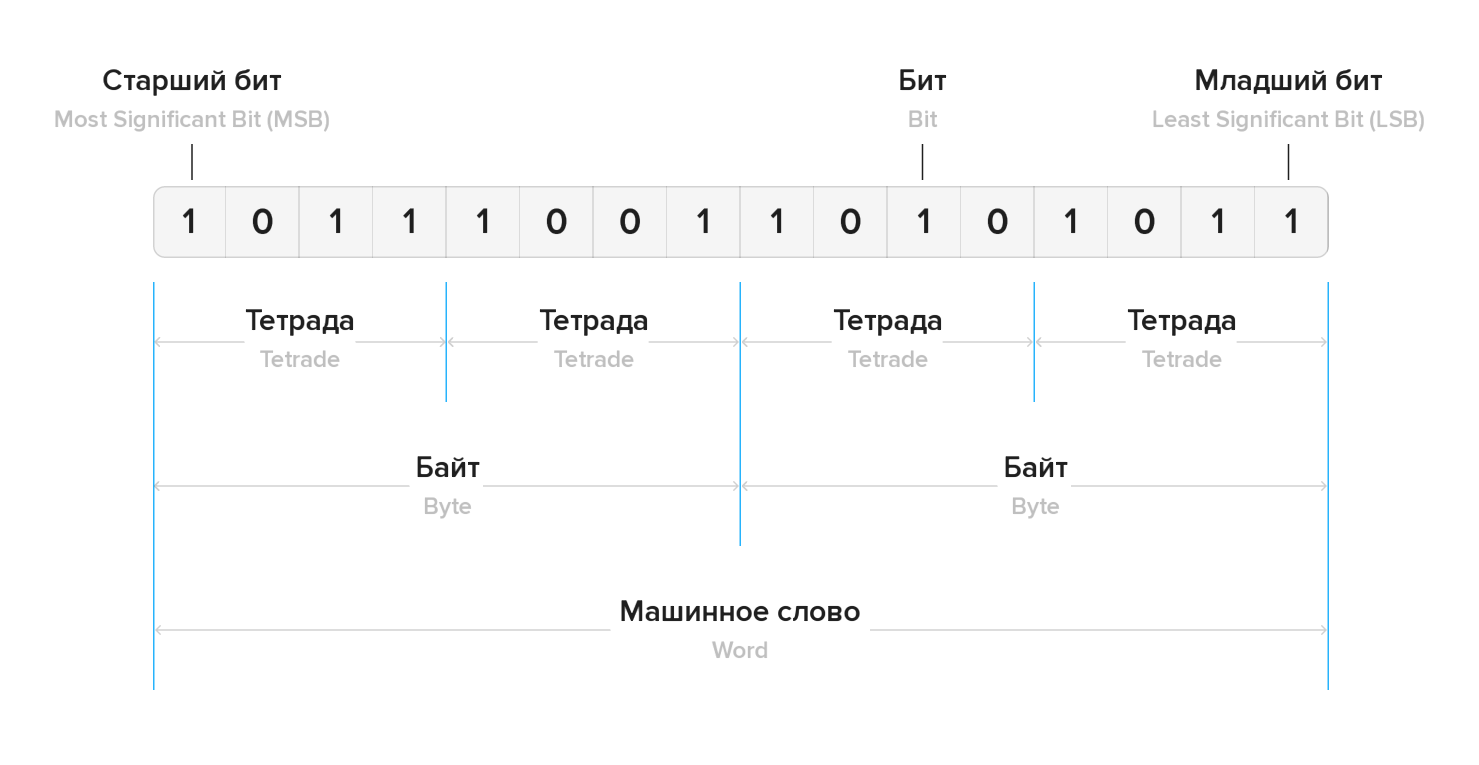
\includegraphics[width=130mm, height=60mm]{/home/llyy/Yandex.Disk/personal/knowledge/general/algorithms_course/repo/algorithms_course/0_intro/images/bit_byte_nibble_word}

\scriptsize Источник - этот курс

\end{frame}

%%%%%%%%%%%%%%%%%%%%%%%%%%%%%%%%%%%%%%%%%%%%%%%%%%%%%%%%%%%%%%%%%%%%%%%%%%%%%%%%%%%%%%%%%%%%%%%%%
\begin{frame}
\frametitle{Алгоритмы и данные}
\framesubtitle{Представление данных}
\justifying
\begin{block}{}
\begin{columns}[]
\column{\dimexpr\linewidth-40mm}
\justifying
\small
Каждую тетраду/полубайт удобно представлять в виде одной цифры в шестнадцатиричной системе счисления, потому что для ее представления 
нужно как раз 4 бита. Двоичные данные, записанные в таком виде обычно называют hex кодами (hexadecimal)\newline

\centering
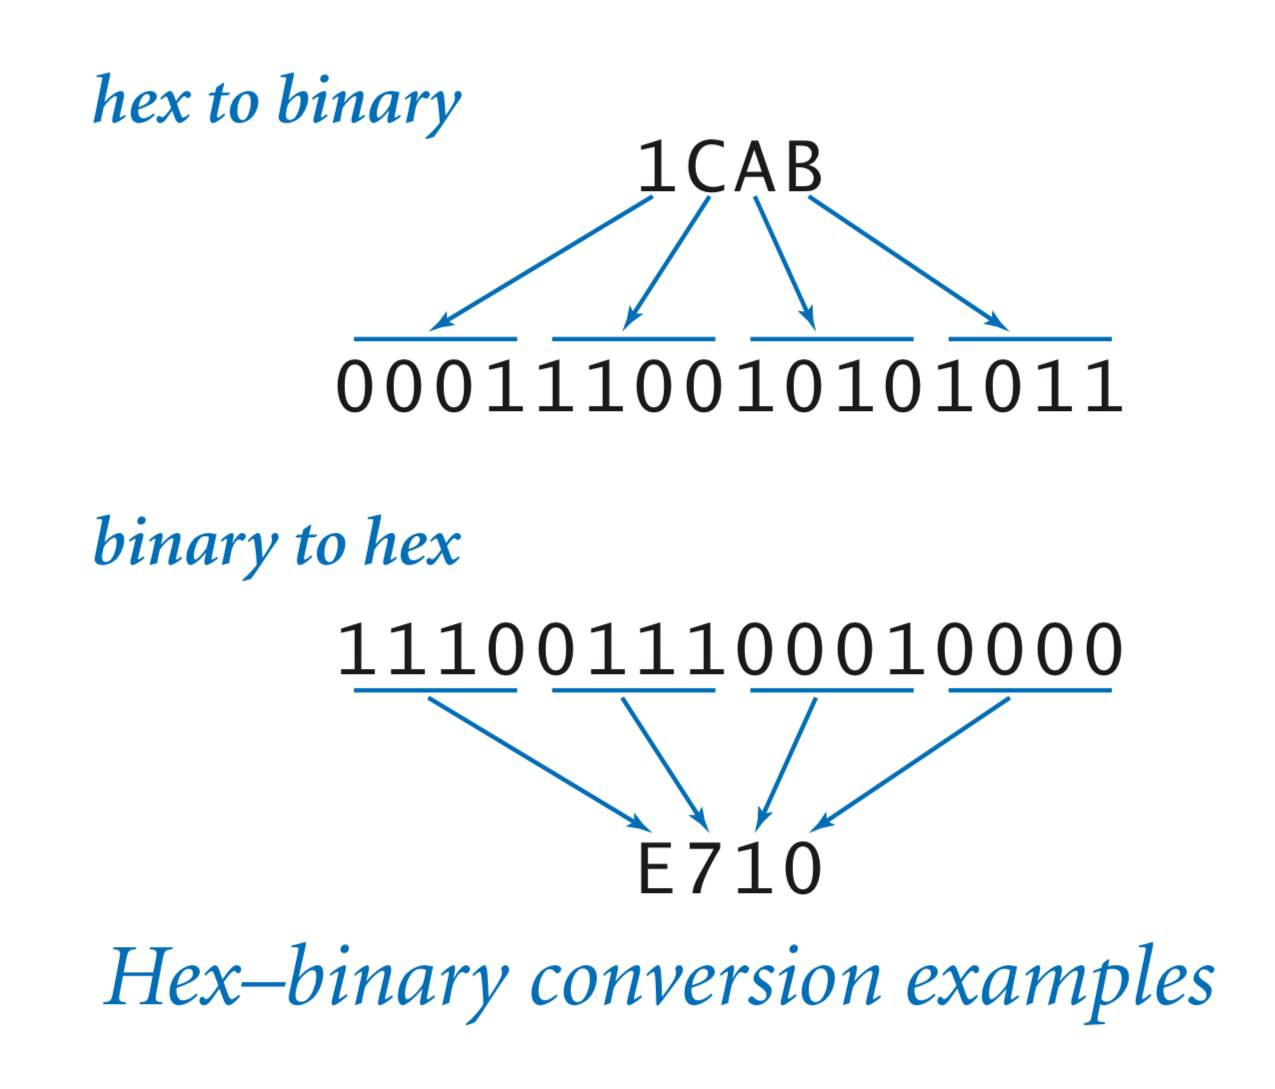
\includegraphics[width=45mm, height=45mm]{/home/llyy/Yandex.Disk/personal/knowledge/general/algorithms_course/repo/algorithms_course/0_intro/images/hex_to_bin_conversion}
\centering

\column{40mm}

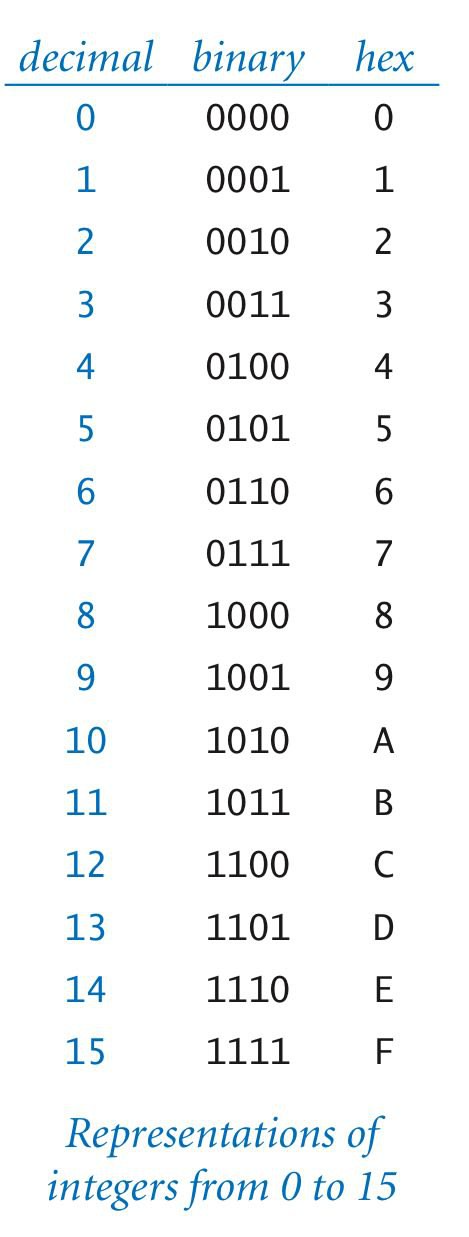
\includegraphics[width=30mm, height=60mm]{/home/llyy/Yandex.Disk/personal/knowledge/general/algorithms_course/repo/algorithms_course/0_intro/images/hex_digits}
\centering


\end{columns}
\end{block}


\end{frame}

\end{document}